\documentclass[12pt,a4paper]{report}																%	Documento A4, corpo 12pt
\usepackage{multirow}
\usepackage[utf8]{inputenc}																		%	Codifica UTF8
\usepackage[italian]{babel}																		% Lingua italiana
\usepackage{csquotes}
\usepackage{amsmath}																			% Funzioni matematiche
\usepackage{amsfonts}																			% Font personalizzati
\usepackage{amssymb}																			% Simboli
\usepackage{graphicx}																			% Immagini
\usepackage{setspace}																			% Modifica interlinea
\usepackage[left=3cm,right=3cm,top=3cm,bottom=3cm]{geometry}										% Impostazione margini
\usepackage{sectsty}																			% Impostazione titoli capitoli e sezioni
\usepackage{float}																				% Per usare option 'H' sulle figure
\usepackage[font=scriptsize,labelfont=bf]{caption}												% Impostazione didascalie
\usepackage{xcolor}																				% Didascalia più articolata
\usepackage{listings}																			% Inserimento codici sorgente
\usepackage{array}
\newcolumntype{L}[1]{>{\raggedright\let\newline\\\arraybackslash\hspace{0pt}}m{#1}}
\newcolumntype{C}[1]{>{\centering\let\newline\\\arraybackslash\hspace{0pt}}m{#1}}
\newcolumntype{R}[1]{>{\raggedleft\let\newline\\\arraybackslash\hspace{0pt}}m{#1}}
\usepackage[
backend=bibtex,
style=numeric,
sorting=none
]{biblatex}																						% Bibliografia						

\addbibresource{Bibliografia.bib}

% Ridefinizione delle didascalie per i codici sorgente
\renewcommand{\lstlistingname}{Codice}
\renewcommand{\lstlistlistingname}{Elenco dei codici}

% Impostazioni globali per sezioni di codici sorgente
\lstset{ 
	language=Matlab,                					%	choose the language of the code
	%	basicstyle=10pt,       						%	the size of the fonts that are used for the code
	numbers=left,                  					%	where to put the line-numbers
	numberstyle=\footnotesize,      					%	the size of the fonts that are used for the line-numbers
	stepnumber=1,                   					%	the step between two line-numbers. If it's 1 each line will be numbered
	numbersep=5pt,                  					%	how far the line-numbers are from the code
	%	backgroundcolor=\color{white},  				%	choose the background color. You must add \usepackage{color}
	showspaces=false,               					%	show spaces adding particular underscores
	showstringspaces=false,         					%	underline spaces within strings
	showtabs=false,                 					%	show tabs within strings adding particular underscores
	frame=single,	                					%	adds a frame around the code
	% tabsize=2,                						%	sets default tabsize to 2 spaces
	captionpos=b,                   					%	sets the caption-position to bottom
	breaklines=true,                					%	sets automatic line breaking
	breakatwhitespace=false,        					%	sets if automatic breaks should only happen at whitespace
	escapeinside={\%*}{*)},          				%	if you want to add a comment within your code
	extendedchars=true,
	literate=
		{è}{{\`e}}1
		{ù}{{\`u}}1
		{ò}{{\`o}}1
		{à}{{\`a}}1
		{ì}{{\`i}}1
}

% Dimensione titolo dei capitoli
\chapternumberfont{\LARGE} 
\chaptertitlefont{\Large}

% Rimozione indentazione inizio paragrafo
\setlength{\parindent}{0in}

% Interlinea 1.5
\onehalfspace

% Global path per le immagini (EPS)
\graphicspath{{figures/}}

% Inizio documento
\begin{document}
	
\begin{titlepage}
		\begin{center}
			
			{
\includegraphics[width=4cm]{logo.pdf}}
			\vspace{0.5cm}
			
			{\LARGE{Politecnico di Bari}}\\
			\vspace{0.5cm}
			
			{\large{Dipartimento di Ingegneria Elettrica e dell'Informazione}}\\
			{\normalsize{Corso di Laurea Triennale in Ingegneria Informatica e dell'Automazione}}\\
			\line(1,0){350}\\
			\vfill
			{\large Tesi in Controllo Digitale}\\
			\vspace{0.5cm}		
			{\large \textbf {
Realizzazione ed implementazione di un algoritmo di controllo di semafori per la gestione ottimizzata del traffico in un modello a più incroci}}\\
		\end{center}
		\vfill
		\begin{minipage}{\textwidth}
			\begin{minipage}{2in}
				\textbf{Relatore:} \\
				Prof. Paolo Lino
			\end{minipage}
			\hfill
			\begin{minipage}{1.3in}
				\textbf{Studente:} \\
				Giorgio Mannarini
			\end{minipage}
		\end{minipage}
		\vfill
		\centering \small {Anno Accademico 2019 - 2020}

\end{titlepage}
% \input{Abstract}
% \input{Dedication}

% Indice, elenco figure, elenco codici
\tableofcontents
\listoffigures
\lstlistoflistings
\listoftables

% Divisione dei capitoli con le relative sezioni
\chapter*{Introduzione}
\addcontentsline{toc}{chapter}{Introduzione}
Il controllo del traffico automobilistico mediante algoritmi performanti, soprattutto per quanto concerne le città più popolose, è un problema affrontato in numerosi documenti di stampo scientifico; tuttavia pochi sono stati i risultati finora raggiunti, ed il sistema più utilizzato per gestire il flusso di veicoli nelle intersezioni stradali resta quello dei semafori staticamente programmati, indipendenti cioè da parametri o eventi esterni.

Certamente negli anni si è compresa quantomeno l’importanza di assegnare una differente priorità, comunque statica, alle varie strade, in modo tale da privilegiare le arterie principali con meccanismi come le onde verdi, tuttavia sarebbe più auspicabile un processo a priorità dinamica, che conceda il verde alle strade più congestionate. Numerose sono le ricerche effettuate in tal senso, sia per quanto concerne l’algoritmo da adottare, che per quanto riguarda la sua relativa implementazione.

In questo lavoro di tesi si è selezionato uno degli algoritmi più comuni, lo si è modificato per migliorarne ulteriormente le performance, e lo si è applicato ad uno scenario di simulazione reale, anch’esso realizzato in maniera autonoma. È da chiarire che l’obiettivo non è stato quello di snellire il traffico quando tutte le arterie che convergono nell’incrocio sono sature di veicoli, quanto più di ottenere buone performance in questa situazione, migliorando molto però il comportamento dei semafori in condizioni di squilibrio, ovvero quando le strade affollate sono solo alcune delle confluenti.

Nello specifico, in primo luogo è stato necessario stabilire la tipologia di incrocio da analizzare, e in tal senso è stata scelta una intersezione a raso a quattro bracci \cite{incrocio}, in cui ogni direzione è percorribile sia in un senso che in quello opposto, e nessuna svolta è vietata. A tal proposito, si è reso fondamentale creare il modello che simula il singolo incrocio in Matlab, Simulink e SimEvents, per monitorare l’andamento del traffico variando alcuni parametri come il tasso di arrivo dei veicoli e la durata del verde, iniziando da un classico algoritmo di gestione statica, implementato comunemente in questo tipo di giunzioni.

Il passo successivo è stato quello di stabilire quali sono le direzioni fra loro compatibili, alle quali cioè è possibile concedere il verde contemporaneamente senza causare incidenti. È da sottolineare che questo lavoro viene normalmente svolto durante il posizionamento e la regolazione di un semaforo classico, e che per ogni tipo di incrocio esistono tabelle indicanti proprio tutte queste direzioni compatibili. La creazione di una tabella di questo genere è il primo passo per la definizione di un algoritmo di gestione ottimizzata dell’incrocio stesso.

Per quanto concerne l’algoritmo ideato, esso si basa su una proposta di \textit{Maram Bani Younes} e \textit{Azzedine Boukerche} \cite{itlc}, modificata ed opportunamente adattata. Si è proceduto dapprima a tradurre l’idea in codice, applicandola ad un singolo incrocio, sfruttando il modello realizzato in precedenza, per poi proseguire con la realizzazione di un modello più complesso e a più ampio respiro, che coinvolge nove diverse intersezioni, collegate fra loro, per simulare una situazione in cui le automobili che lasciano una giunzione confluiscano nella successiva.

A tal proposito, si è reso opportuno modificare ancora una volta l’algoritmo, per adattarlo ad una situazione di questo genere, ed i dati ricavati sono stati confrontati con quelli provenienti dallo stesso modello a nove incroci, gestito però con una turnazione classica dei semafori.

Nel \textbf{capitolo 1} viene dunque introdotto il primo modello realizzato, quello del singolo incrocio, e ne vengono analizzate le performance al variare del tasso di generazione delle auto e alla durata del verde per ciascuna strada, senza l’utilizzo di un algoritmo a priorità dinamica.

Nel \textbf{capitolo 2} viene esplicato il funzionamento dell’algoritmo sopracitato, le modifiche apportate, e viene mostrato come la sua applicazione al modello precedente, a parità di altre condizioni, migliori le performance dell’incrocio, misurate in termini di numero di auto in coda e tempo di attesa medio delle stesse.

Nel \textbf{capitolo 3} viene presentato il secondo modello realizzato, relativo ad una situazione con nove incroci interconnessi, e ne vengono analizzate le prestazioni in assenza di un algoritmo di controllo.

Nel \textbf{capitolo 4}, in fine, si analizza il comportamento di tale modello in presenza di un algoritmo che tenga conto del numero di auto in coda in ciascuna corsia, e di altri parametri esterni, confrontando i risultati ottenuti con quelli del capitolo precedente.


% Inizio capitolo
\chapter{Modellazione e gestione statica del singolo incrocio \label{capitolo1}}
Come accennato nell’introduzione, è stato scelto di analizzare un incrocio a raso a quattro bracci, senza limitazioni in termini di svolte e direzioni percorribili. Questo significa che la giunzione, composta appunto da quattro strade disposte nella classica forma a croce, presenta quattro corsie per ogni strada. Per comodità e per adottare una convenzione di linguaggio, ci si riferirà alle automobili che non hanno ancora superato l’incrocio definendole “entranti”, chiamando invece “uscenti” le vetture che già sono passate attraverso la giunzione.

Le quattro corsie, dunque, sono così assegnate: due sono dedicate a veicoli uscenti, provenienti cioè da una delle altre tre strade dell’incrocio, mentre le altre due sono dedicate alle automobili entranti. Nello specifico, adottando una convenzione di “guida a destra”, comune nella maggior parte dei paesi europei, la corsia più a destra delle due entranti è riservata a chi vuole svoltare a destra o andare dritto, mentre quella più a sinistra a coloro i quali vogliono svoltare a sinistra.

Questa suddivisione è molto comune negli incroci italiani, ed è la soluzione più utilizzata nella assegnazione dei sensi di marcia in incroci di questo genere.

Le corsie a cui può essere concesso il verde contemporaneamente sono sempre e solo due, e per ogni corsia ne esistono due possibili complementari, che possono cioè essere scelte per ottenere il verde assieme alla corsia suddetta. La figura in basso è riassuntiva di questo modello, che è applicabile alla tipologia di incrocio scelto ed è indipendente dal tipo di algoritmo utilizzato per controllare i semafori.

Nella gestione ordinaria degli incroci stradali solo una delle due alternative è scelta, in maniera statica, per ogni corsia, in base al flusso di traffico che si prevede per ciascun senso di marcia.

\begin{figure}[H]
	\centering
	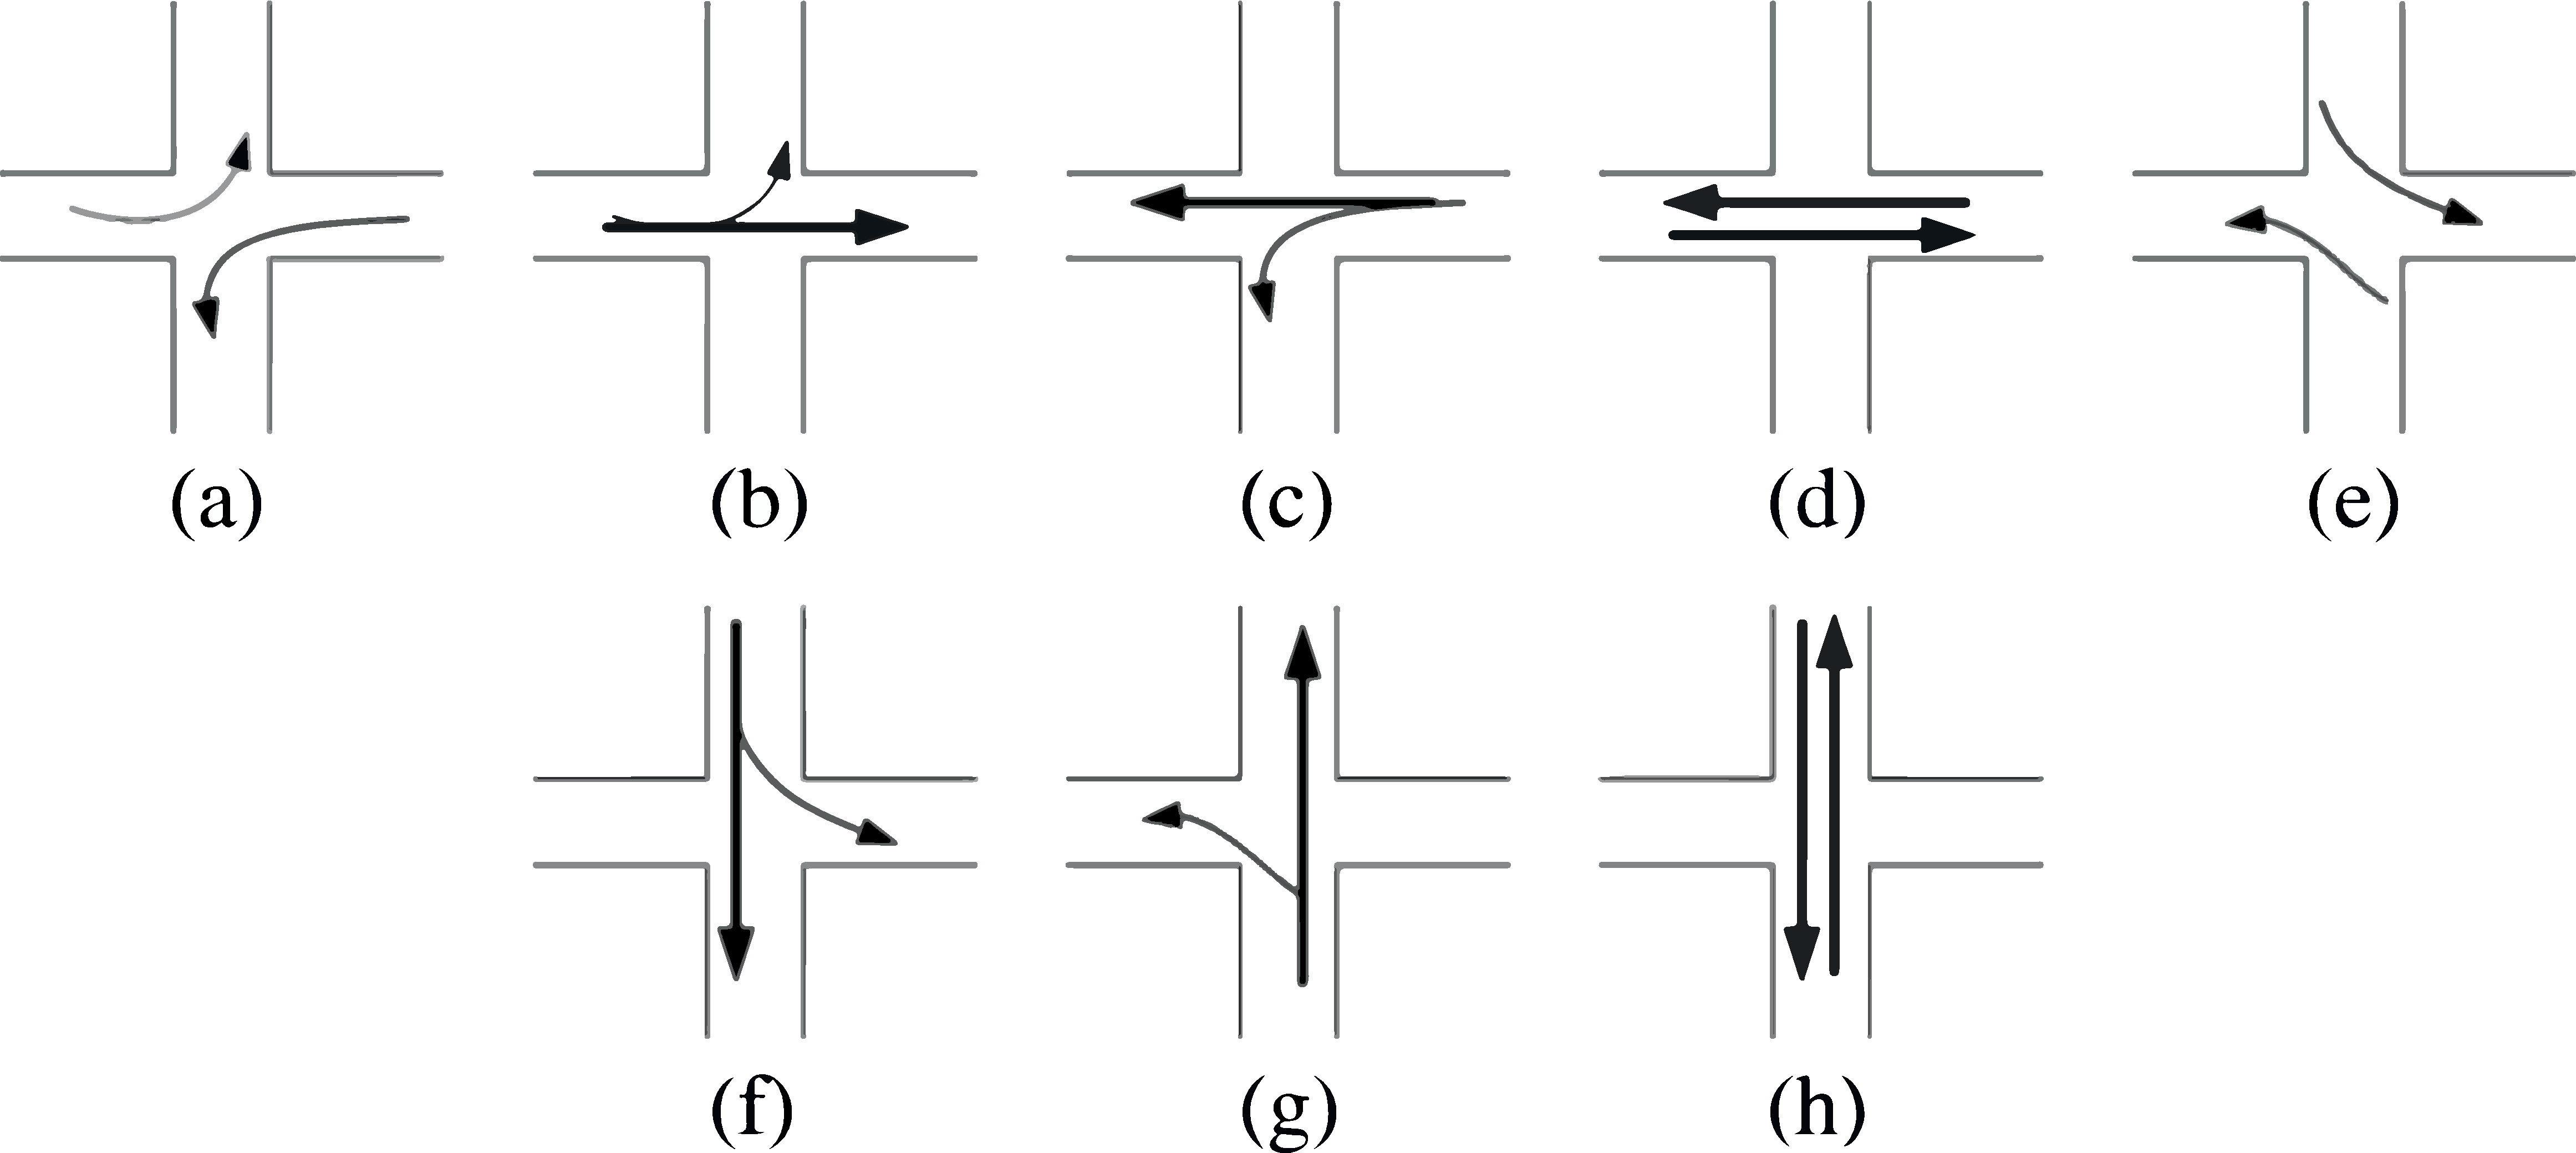
\includegraphics[width=1\textwidth]{compatibili.pdf}
	\caption{Direzioni compatibili}
	\label{dirCompatibili}
\end{figure}
\label{figure: DirezioniCompatibili}
Nel modello oggetto di questo primo capitolo, è stato scelto di concedere il verde alle due corsie facenti parte della stessa strada, quella per svoltare a sinistra e quella per svoltare a destra / andare dritto, ovviamente a turno, per ognuno dei quattro bracci dell’incrocio (schemi (b), (c), (f), (g)). Ciò tuttavia non esclude che, essendo il sopracitato modello profondamente personalizzabile e parametrizzato, si possa prevedere anche la seconda opzione, indicata dagli schemi (a), (d), (e), (h) in figura.

\newpage
\section{Generazione delle automobili}
Per quanto concerne la generazione delle auto, questa è indipendente per ogni corsia ed avviene mediante un processo di Poisson, utilizzato nella maggior parte dei modelli di simulazione del traffico \cite{probability}. Se di tale processo stocastico si è interessati alla probabilità che il tempo trascorso tra due eventi consecutivi sia pari a t è necessario fare ricorso ad una distribuzione esponenziale, di parametro t, la cui funzione densità di probabilità $ f(t)$ in questione, nello specifico, è la seguente.

\begin{equation}
PDF: f(t) = \lambda e^{\lambda t}
\end{equation}
Gli Entity Generator di Simulink, gli oggetti utilizzati per generare le automobili, prevedono tuttavia che la funzione che li governa sia riferita a $dt$, ovvero all’intervallo di tempo fra due eventi consecutivi, che deve essere una variabile casuale, e non alla sua funzione densità di probabilità. Pertanto, per ricavare tale intervallo di tempo dalla funzione densità di probabilità in oggetto, si fa riferimento alla sua funzione di distribuzione $F(t)$, ottenuta integrando $f(t)$ nell'intervallo $[0, t]$ e che rappresenta la probabilità che in tale intervallo si sia verificato un evento, in questo caso l’arrivo di un’automobile. Tale funzione di distribuzione ha la seguente espressione.
\begin{equation}
CDF: F(t)  = 1-e^{-\lambda t}
\end{equation}
Da essa è facile ricavare la variabile $t$, che rappresenta l’incognita del problema, come inversa della $CDF$.
\begin{equation}
CDF^{-1}: t = -\frac{1}{\lambda} \ln{[1 - F(t)]}
\end{equation}
Nello specifico $F(t)$, che, come già detto, è la probabilità che in un certo intervallo di tempo si verifichi un evento, è scelta casualmente mediante una distribuzione uniforme, fra 0 e 1. Pertanto, se $F(t)=1$ si ha la certezza che c’è stato un arrivo, e questo può essere vero solo se $t \to +\infty$, al contrario per $F(t)=0$ si è sicuri che non si sia verificato alcun evento, e ciò avviene solo se $t \to 0$.

Si nota, dunque, che più aumenta $t$, più è probabile che arrivi un’auto nella corsia in questione. Il tutto è governato dal parametro $\mu = \frac{1}{\lambda}$, arbitrariamente impostabile.

Tale funzione è stata quindi implementata negli Entity Generator, che come già accennato si occupano di generare, appunto, entità, oggetti con determinate caratteristiche controllate dai due toolbox, Simulink e SimEvents.

Per rendere ancora più variabile e casuale il tempo medio che intercorre fra l’arrivo di un’auto e quello della successiva, il parametro $\mu$, e dunque il tasso di generazione delle vetture viene originato randomicamente ad ogni esecuzione, in un intervallo precedentemente determinato, utilizzando questa volta una distribuzione uniforme, capace dunque di assicurare assoluta equi-probabilità. Inoltre, poiché si prevede che durante le ore del giorno il numero di veicoli vari sensibilmente fra le ore di punta, le ore notturne e quelle intermedie, è stato anche previsto un meccanismo per permettere a SimEvents di rilevare in quale ora del giorno si trova durante la simulazione, e aumentare o diminuire di conseguenza $\mu$. In definitiva, il codice utilizzato per la generazione delle automobili è alla seguente pagina.
\newpage
\begin{lstlisting}[language=Matlab,label=entity-generator,caption=Entity Generator]
%Random number generation

coder.extrinsic('rand');
ValEntry1 = 1;
ValEntry1 = rand();
%ValEntry1 rappresenta la CDF

index = 1;
%indice del generator, in questo caso il primo.

% Ora del giorno
time = mod(getTime(), 86400) / 3600;

% Fasce orarie
if time > 0 && time < 7
myMu = muNotte(index);
elseif time > 7.5 && time < 9
myMu = muMattinaPranzo(index);
elseif time > 12 && time < 14.5
myMu = muMattinaPranzo(index);
elseif time > 18 && time < 20
myMu = muSera(index);
else
myMu = muArray(index);
end

% Pattern: distribuzione esponenziale 
dt = -myMu * log(1 - ValEntry1);
% dt: tempo fra due eventi di Poisson
\end{lstlisting}
\newpage
Come è facile comprendere, si ha, rispetto alla descrizione precedente, $\mu = myMu$.

È inoltre da precisare che i parametri $muNotte$, $muMattinaPranzo$, $muSera$ e $muArray$ sono definiti come variabili globali, con questo codice.

\begin{lstlisting}[language=Matlab,label=mu-definition,caption= Tassi di generazione variabili]
coder.extrinsic('rand');
temp = 1;
temp = rand([1 8]);
%creo 8 numeri casuali fra 0 e 1, uno per ogni generator
muArray = 20 + (35 - 20) * temp;
%l'intervallo scelto va da 20 a 35

muNotte = muArray + 80; %di notte il tasso è molto basso
muMattinaPranzo = muArray - 6; %di mattina ed a pranzo è molto alto
muSera = muArray - 3; %di sera è più alto del normale
\end{lstlisting}

Per definire delle variabili globali è necessario accedere al \textit{Model Workspace} mediante il pulsante in basso a sinistra in \textit{figura \ref{fig:accesstoworkspace}}. Una volta fatto ciò, spostandosi sul modello (in questo caso \textit{GateControl}), e sulla tab \textit{Callbacks} in alto a destra, è possibile inserire il codice appena presentato cliccando su \textit{InitFcn}, ovvero lo spazio in cui possono essere dichiarate le funzioni / variabili di inizializzazione del modello.

\begin{figure}[H]
  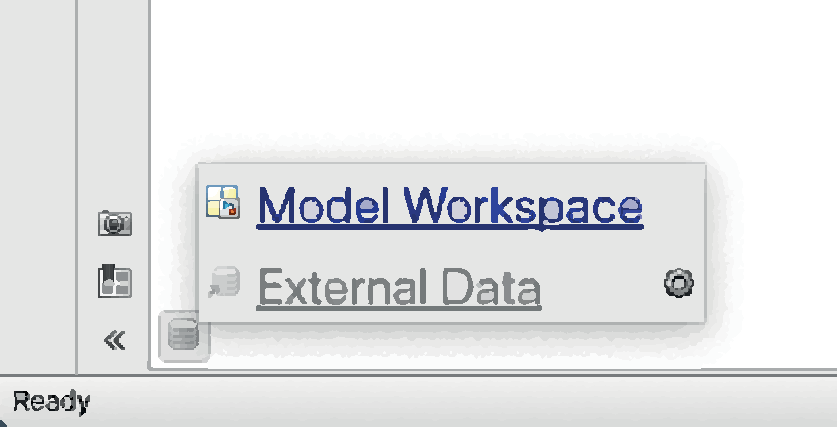
\includegraphics[width=1\textwidth]{accessToWorkspace.pdf}
  \caption{Accesso al workspace, ingrandimeto}
  \label{fig:accesstoworkspace}
\end{figure}

\begin{figure}[H]
  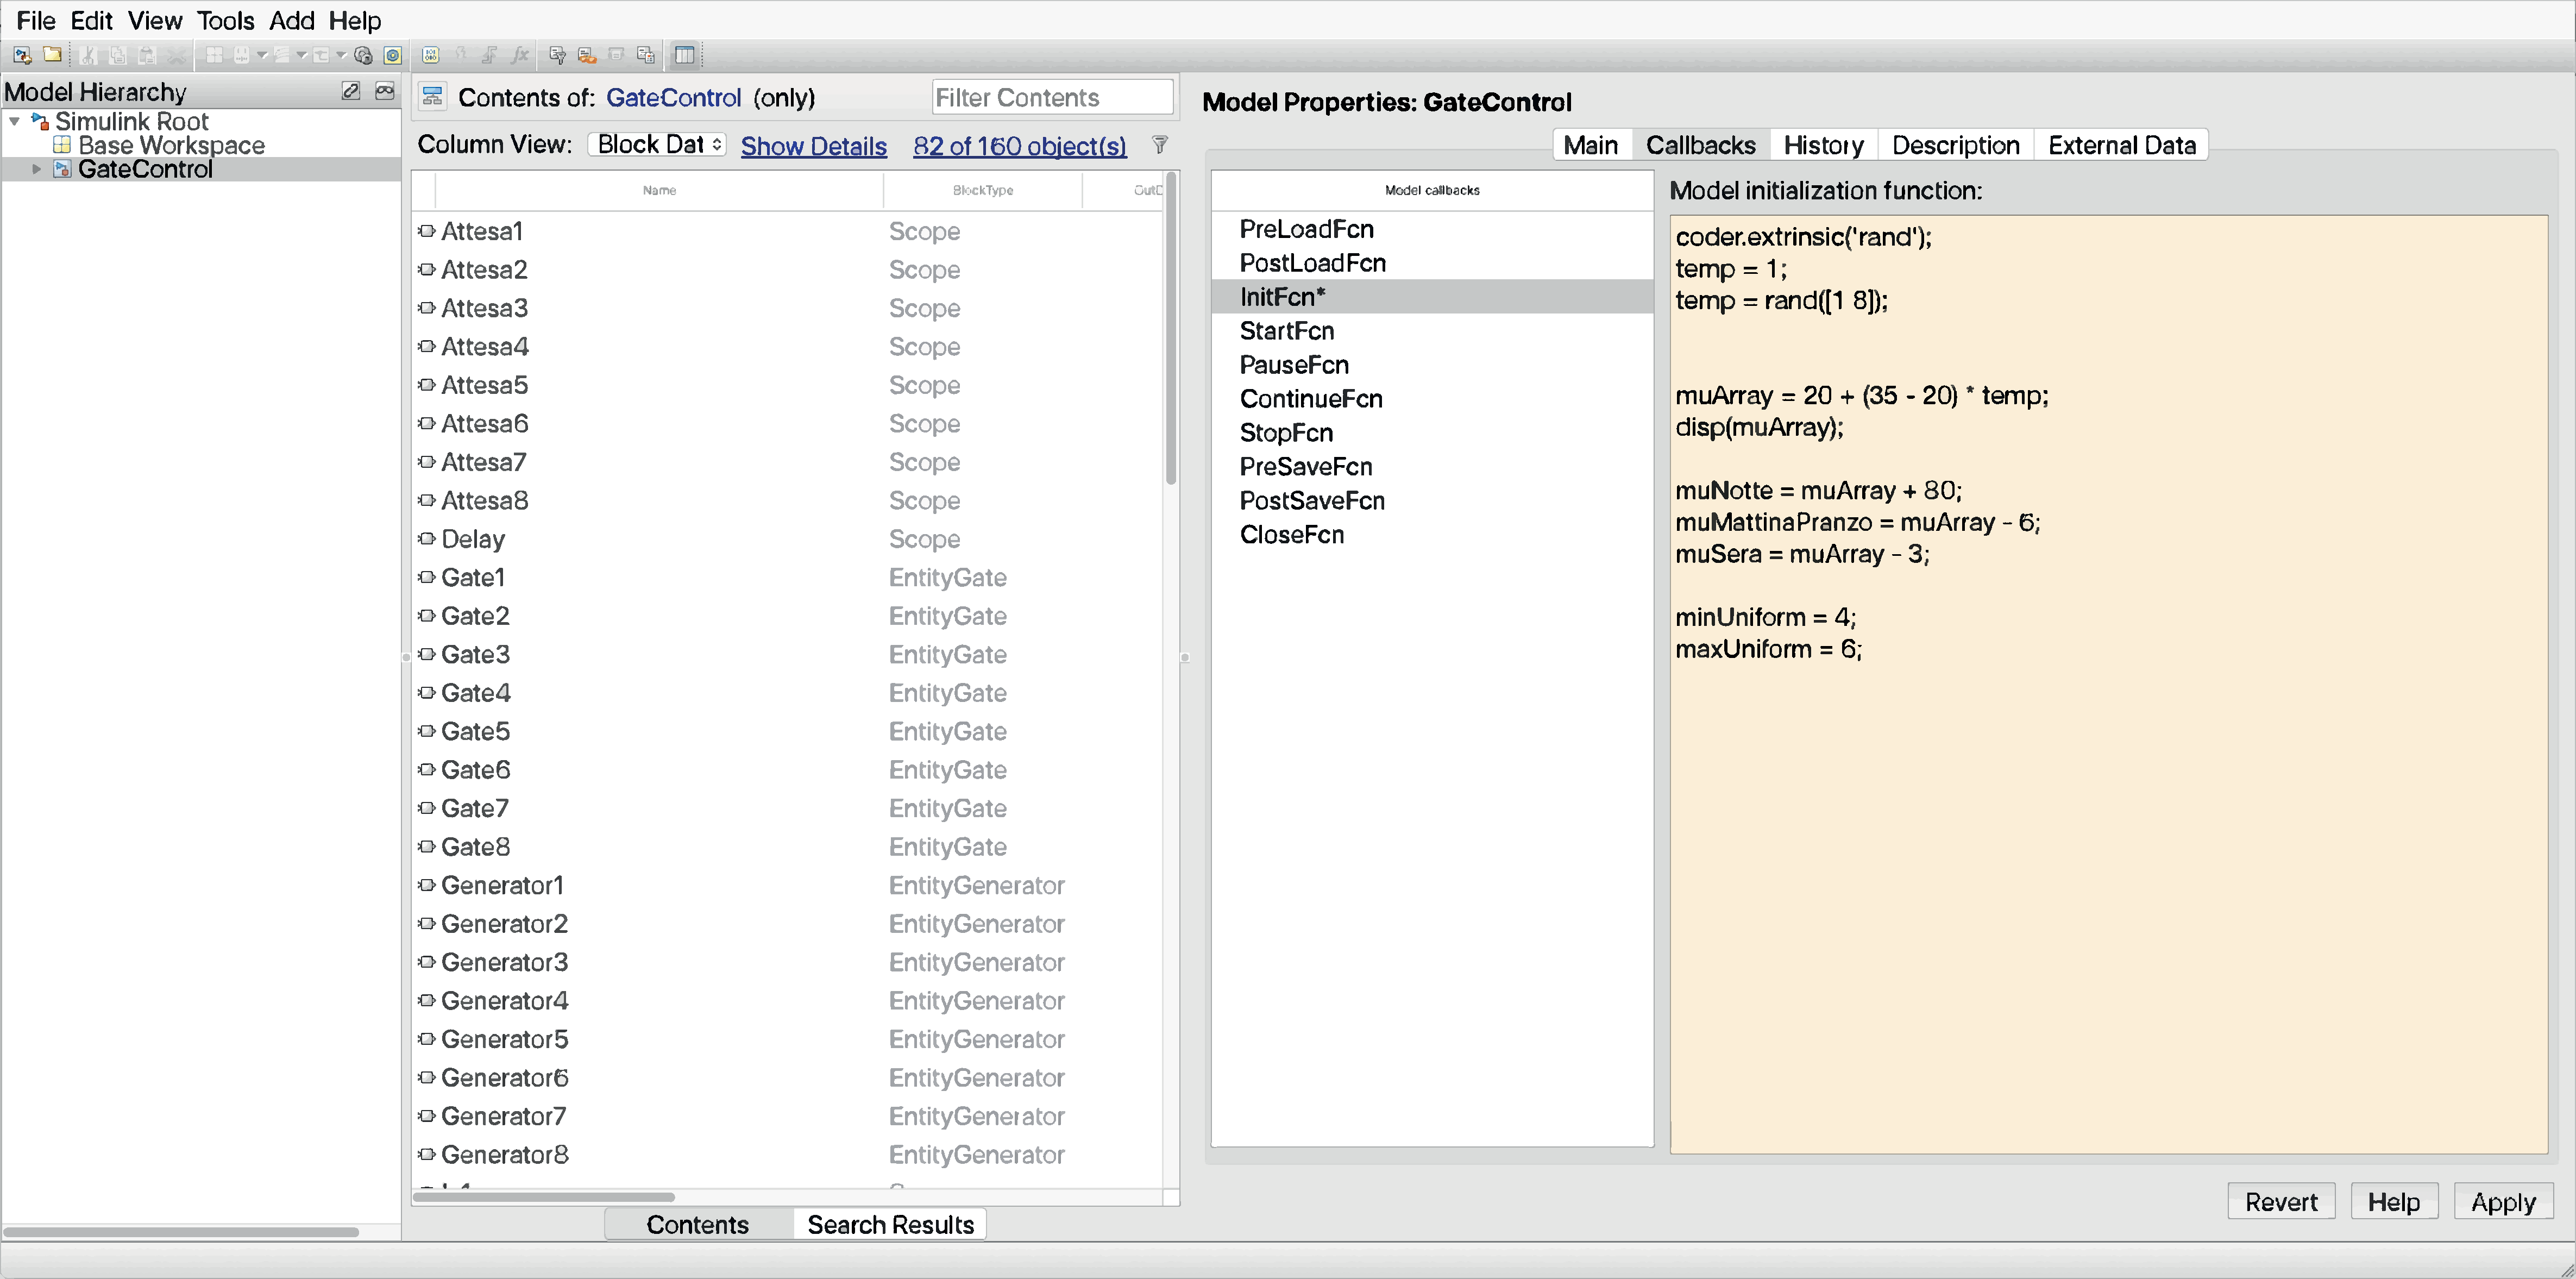
\includegraphics[width=1\textwidth]{InitFcn.pdf}
  \caption{Inserimento di variabili globali e codice di inizializzazione nel modello}
  \label{fig:initfcn}
\end{figure}

Si può notare dal \textit{codice \ref{mu-definition}} che vengono generati otto numeri casuali, fra 20 e 35, che costituiscono i valori base per il parametro $\mu$. Ciò vuol dire che mediamente fra l’arrivo di un’auto e della successiva intercorre un tempo compreso tra:
\begin{equation*}
	dt = -20 \ln{[1 - 0.5]} = 13.86s
\end{equation*} 
\begin{center}
	e
\end{center}
\begin{equation*}
dt = -35 \ln{[1 - 0.5]} = 24.26s
\end{equation*}
dove 0.5 è il valore medio della distribuzione uniforme precedentemente descritta. Tali valori base sono utilizzati nelle ore intermedie, come già detto, mentre sono modificati durante le ore di punta e quelle notturne.

Il valore di $\mu$ è poi profondamente decrementato durante le ore di punta (mattina e ora di pranzo), incrementato durante la notte e decrementato, anche se meno drasticamente, all’ora di cena, influendo ovviamente sui tempi di interarrivo, che diventano i seguenti.

\textbf{Mattina e pranzo} (fra le ore 7.30 e le ore 9.00, e fra le ore 12.00 e le ore 14.30): da 9.7 secondi a 20.1 secondi.

\textbf{Sera} (fra le ore 18.00 e le ore 20.00): da 11.78 secondi a 22.18 secondi.

\textbf{Notte} (fra le ore 0.00 e le ore 7.00): da 69.31 secondi a 79.71 secondi.

Il tutto è stato fatto per rendere il modello quanto più imprevedibile possibile, mantenendolo però fedele alla realtà.

Si nota che, con questi tassi, vengono mediamente generate 2200 automobili per ogni corsia, ovvero circa 17600 vetture attraversanti l’incrocio durante l’arco di 24 ore, come riportato dal seguente grafico.

\begin{figure}[H]
	\centering
	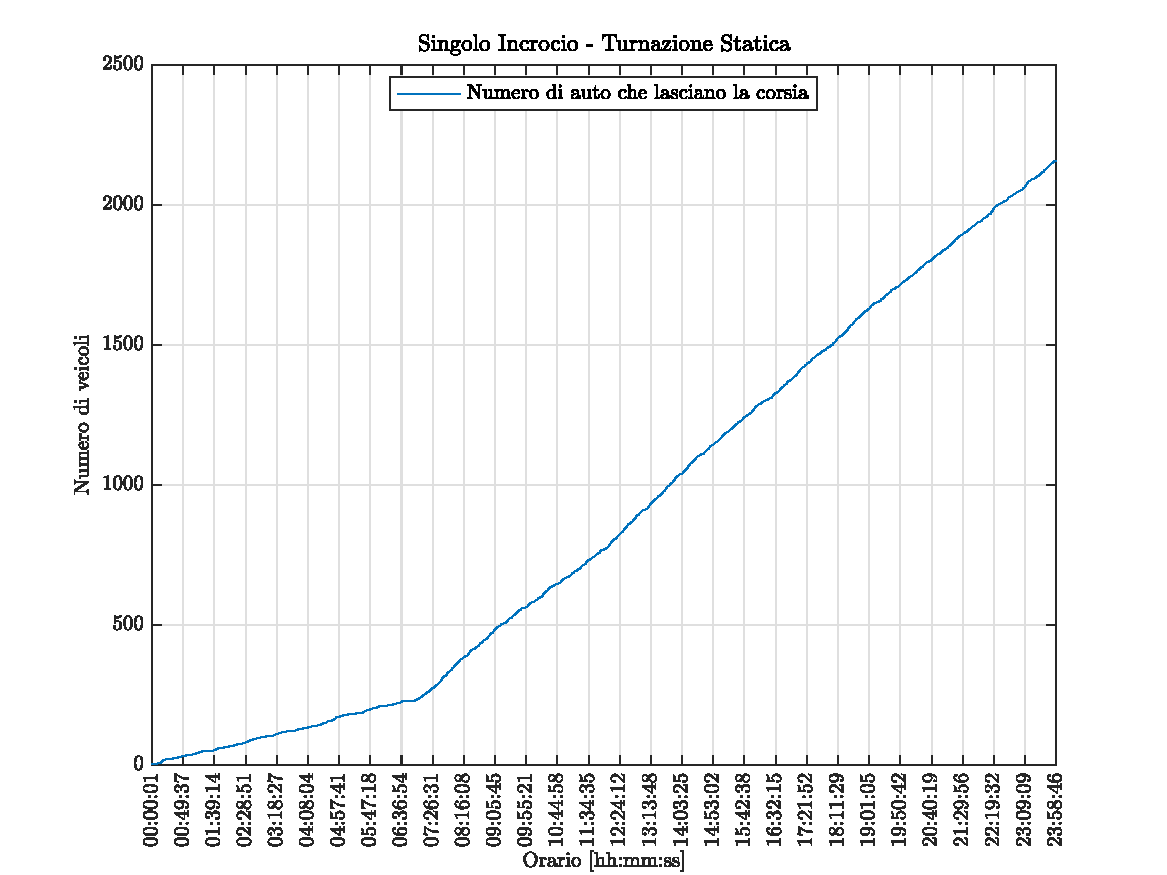
\includegraphics[width=1\textwidth]{AutoTotaliStatico.pdf}
	\caption{Vetture complessive nell'arco di 24 ore per una singola corsia}
\end{figure}
\newpage

La scelta di questi valori non è stata casuale: si è voluto infatti considerare il caso di un’intersezione affollata, plausibile nelle grandi città. Variando il parametro manualmente e sperimentando rispetto al numero di automobili, si è trovato in questi numeri un buon compromesso per analizzare il comportamento del modello e dell’algoritmo applicato. 

È infatti da notare che negli incroci in cui mediamente il numero di veicoli giornalieri è molto basso l’applicazione di un algoritmo di controllo come quello che sarà presentato nel capitolo successivo di questo lavoro di tesi risulta sì essere utile, ma meno drasticamente determinante, in quanto non vi è una situazione di traffico intenso e di profondo squilibrio, con strade molto affollate e strade con poche automobili, situazione che invece verrà ricreata, in seguito, per confrontare l’algoritmo statico di questo capitolo con quello dinamico, di cui si discuterà. 

Anche le variazioni in base alle fasce orarie sono state analizzate, e non lasciate al caso: si è voluto infatti simulare un pesante congestionamento nelle ore del giorno mediamente più critiche per una giunzione strategica di una città, ossia fra le ore 7.30 e le ore 9.00, quando gli alunni prendono posto in classe ed i lavoratori arrivano nei loro uffici, così come fra le ore 12.00 e le ore 14.30, e in serata, fra le ore 18.00 e le ore 20.00. Si è considerato, tuttavia, che in quest’ultima fascia oraria, complice l’assenza dei bambini, ormai a casa, e di molti anziani, il tasso sia sì più elevato rispetto a quello standard, per via dei lavoratori, di ritorno alle loro abitazioni, ma meno rispetto a quello mattutino e dell’ora di pranzo.
Durante la notte, invece, si è voluto mantenere il numero di veicoli molto basso, anche questa volta facendo riferimento ad un grande incrocio cittadino. 

Quindi in definitiva i valori di $\mu$ sono frutto di simulazioni sperimentali e di un compromesso fra una situazione realmente plausibile ed un congestionamento dell'incrocio comunque elevato.

Per concludere, la seguente tabella è riassuntiva rispetto ai valori di $\mu$ scelti in base all’ora del giorno ed ai relativi tempi di inter-arrivo. Nel paragrafo conclusivo di questo capitolo, a tale tabella verranno aggiunti anche i tempi medi di attesa di ciascuna automobile nonché il numero medio di auto in coda per ciascuna corsia, e sarà certamente più chiara la corrispondenza fra il parametro ed il flusso di autovetture.
\newpage

\begin{table}[H]
\centering
\begin{tabular}{|c|c|C{3.7cm}|C{3,7cm}|}
  \hline
  \textbf{Fascia Oraria} & 
  \textbf{Intervallo $\mu$} & 
  \textbf{Stima tempo minimo fra due arrivi} & 
  \textbf{Stima tempo massimo fra due arrivi} \\\hline
  0.00 - 7.00 & 
  100 - 115 & 
  69.31s & 
  79.71s \\\hline
  7.00 - 7.30 & 
  20 - 35 & 
  13.86s & 
  24.26s \\\hline
  7.30 - 9.00 & 
  14 - 29 & 
  9.7s & 
  20.1s \\\hline
  9.00 - 12.00 & 
  20 - 35 & 
  13.86s & 
  24.26s \\\hline
  12.00 - 14.30 & 
  14 - 29 & 
  9.7ss & 
  20.1s \\\hline
  14.30 - 18.00 & 
  20 - 35 & 
  13.86s & 
  24.26s \\\hline
  18.00 - 20.00 & 
  17 - 32 & 
  11.78s & 
  22.18s \\\hline
  20.00 - 0.00 & 
  20 - 35 & 
  13.86s & 
  24.26s \\\hline
\end{tabular}
\caption{Relazione fra il parametro $\mu$ ed i tempi di interarrivo}
\label{table:tabellatempiinterarrivo}
\end{table}
È importante anche indicare la presenza di lassi temporali intermedi, fra un cambiamento ed un altro, come quello relativo alla fascia oraria 7.00 – 7.30, in cui il valore di $\mu$ viene posto al valore standard, che rappresenta a tutti gli effetti una “via di mezzo” fra la stima precedente e la successiva. Questo per non provocare un cambiamento troppo repentino del tasso di arrivo dei veicoli, inverosimile nella realtà, in cui aumenta e diminuisce gradualmente. 


\newpage
\section{Il modello in Simulink e SimEvents: introduzione}
Per quanto concerne il resto del modello, come si può notare nella figura seguente, ogni strada è rappresentata, oltre che dall’Entity Generator relativo, da una coda di tipo FIFO (First In First Out), la cui capienza può essere variata a piacimento, da un Entity Gate, che rappresenta il semaforo, e che dunque può assumere lo stato di \textit{chiuso} (semaforo rosso) o \textit{aperto} (semaforo verde), da un Entity Server, utile per modellare il tempo che una singola macchina trascorre nell’incrocio vero e proprio, quindi da quando lascia la strada da cui proviene a quando imbocca quella di uscita, ed in fine da un Entity Terminator, che non fa altro che eliminare dal modello i veicoli che hanno già lasciato l’incrocio.

\begin{figure}[H]
	\centering
	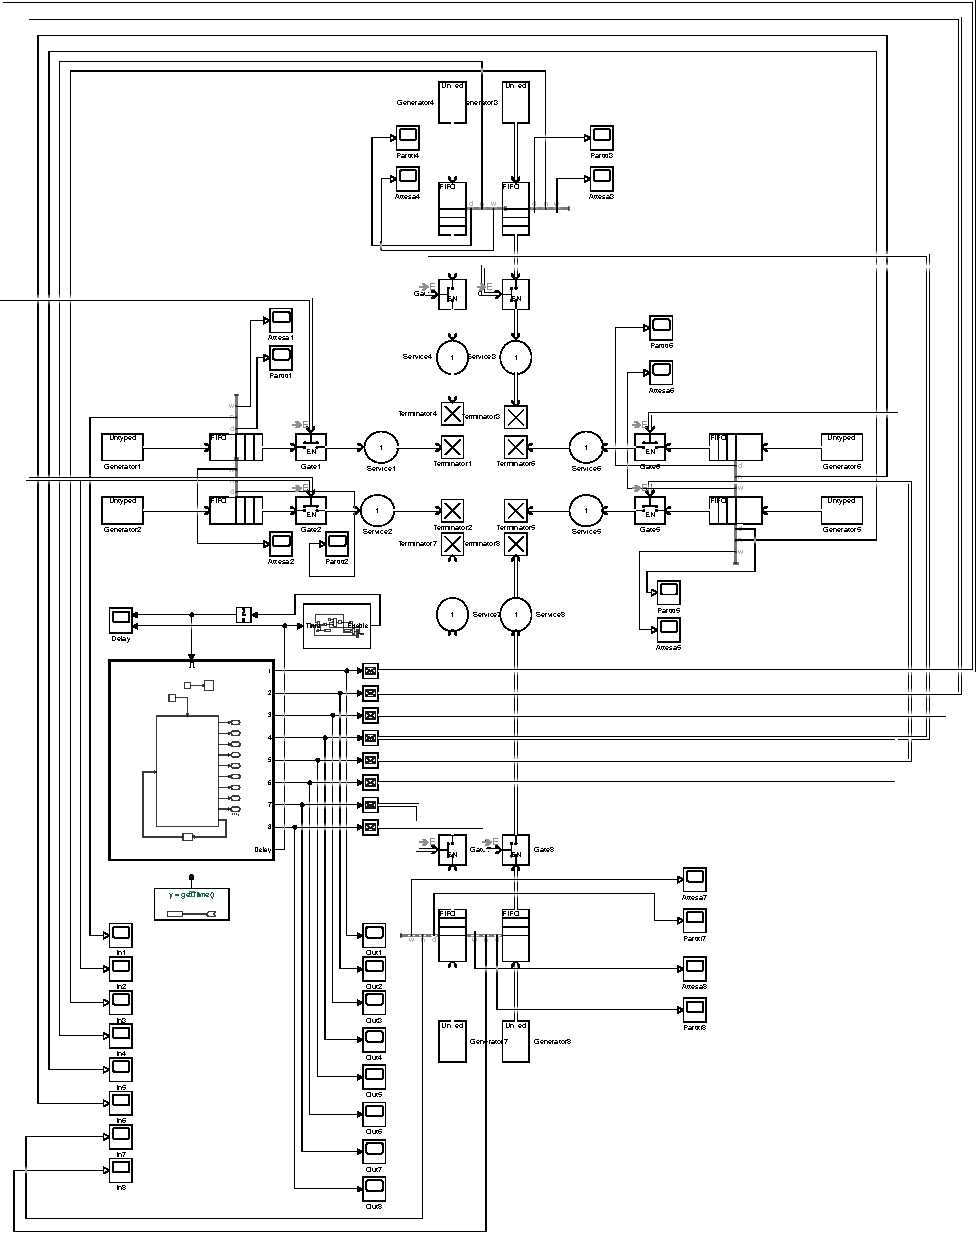
\includegraphics[width=0.75\textwidth]{ModelloSingoloIncrocio.pdf}
	\caption{Modello di un incrocio a raso a quattro bracci in Simulink e SimEvents, gestione statica}
	\label{fig: modelloSingoloIncrocio}
\end{figure}
\newpage
Sono da fare alcune importanti precisazioni:
\begin{enumerate}
	\item La grandezza delle code è stata impostata ad infinito, questo per valutare l’efficienza dei due algoritmi e non avere risultati falsati dati dal fatto che le code si riempiono. In altre parole, non ci sono limiti, in questo modello, a quante macchine possono essere presenti in una singola corsia, tuttavia questi limiti possono essere tranquillamente imposti per poter rendere lo schema più fedele alla realtà. Ciò vale esclusivamente per il modello a singolo incrocio, per i motivi suddetti. Nel Capitolo 3 verrà introdotto un nuovo modello, con più incroci interconnessi, e questo, per adattarsi meglio al funzionamento reale, sarà proposto con code che presentano una capienza massima, condizionata dalla distanza della giunzione in questione da quella precedente.
	\item Il tempo che una macchina trascorre al centro dell’incrocio, definito all’interno degli Entity Server, ha una componente casuale, in quanto si è osservato che anche questo parametro, nel mondo reale, non è fisso, e si è voluta inserire un’ulteriore variabile di imprevedibilità nel modello. Nello specifico si è utilizzata una distribuzione uniforme in un intervallo [4, 6] secondi, come si può notare anche nel \textit{codice \ref{parametri-globali-server}} inerente alla spiegazione specifica del componente in questione. Questi valori non sono casuali: si è voluto stimare il tempo che una macchina impiega ad abbandonare l’incrocio. Considerando che la prima automobile della coda è la più lenta, mentre l’ultima sarà certamente la più veloce, è stato necessario stimare un valore medio. Tale stima resta confinata in un intervallo ristretto perché si è voluto mantenere un valore medio di 5s, senza peggiorare il valore limite superiore, essendo piuttosto inverosimile che un’automobile impieghi più di 6s da quando entra nella giunzione a quando ne esce, in assenza di cause esterne.
	\item È da approfondire anche il concetto della luce gialla: il giallo, infatti, indica alle macchine che non hanno ancora superato il semaforo di fermarsi, e a quelle che stanno occupando l’incrocio di sgomberarlo al più presto. Questo, in effetti, è implicitamente implementato: quando l’Entity Gate si chiude, le macchine al centro dell’incrocio lo liberano, essendo già all’interno dell’Entity Server, consentendo poi a quelle provenienti dalle altre corsie di fluire.
\end{enumerate}
\begin{figure}[H]
  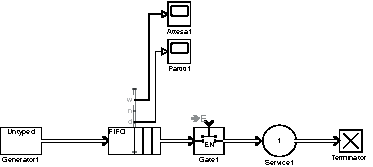
\includegraphics[width=1\textwidth]{catena.pdf}
  \caption{Ingrandimento su una singola corsia}
  \label{fig:catenaSingolaCorsia}
\end{figure}
Oltre ai numerosi oscilloscopi presenti, utili a visualizzare l'evoluzione nel tempo di una serie di informazioni, come il numero di macchine in ogni coda, la durata del verde per ciascun semaforo, il numero di macchine totali che hanno attraversato ogni corsia, il tempo medio d’attesa di ogni corsia, è da sottolineare che l’intero incrocio è governato da un blocco di tipo Enabled Subsystem, all’interno del quale è stata inserita una funzione Matlab, in un blocco Function-Call Subsystem. Ciò che questo blocco consente, è di eseguire tale funzione, una sola volta, solo quando viene inviato un segnale di trigger.

In altre parole, la funzione si occupa di cambiare lo stato del sistema (dare il rosso ai semafori attualmente verdi e concedere il verde ai successivi, per ora staticamente), e deve essere eseguita solo quando effettivamente il tempo concesso alla luce verde dalla chiamata precedente si esaurisce.

A tale scopo, il trigger è gestito da un timer, oggetto non presente in alcuna libreria, che si è prodotto in autonomia. Questo timer accetta in ingresso il tempo, in secondi, per il quale deve restituire in uscita 0, che equivale a \textit{trigger inattivo}, capisce da SimEvents il numero di secondi passati dall’ultima chiamata, e ad ogni passo di campionamento (ogni secondo), esegue il confronto fra questo dato e quello in input, riuscendo così a richiamare la funzione ad intervalli temporali desiderati e ben precisi.
Attualmente questo meccanismo sembra esageratamente complesso, in quanto i semafori hanno delle tempistiche prefissate, che saranno più chiare nel \textit{paragrafo \ref{section: AlgoritmoStatico}}, dedicato alla spiegazione dell’algoritmo di questo primo capitolo, tuttavia in previsione dell’implementazione di una politica di decisione dinamica, sia per quanto concerne le direzioni a cui assegnare il verde, che per la durata dello stesso, si è reso necessario adottare questo tipo di oggetto.
\newpage
\section{Il modello in Simulink e SimEvents: analisi dettagliata dei componenti}

Come accennato in precedenza, la \textit{figura \ref{fig:catenaSingolaCorsia}} è riassuntiva di come è stata modellata una singola corsia. Nello specifico verrà proposta in questo paragrafo una spiegazione più dettagliata di ogni componente.
\newline

\textbf{Entity Generator\cite{entitygen}:} serve a generare entità. Le entità in Simulink e SimEvents sono oggetti con determinate caratteristiche, che possono muoversi all’interno del modello fra componenti collegati fra di loro. In questo caso le entità rappresentano le vetture. 

Ogni entità è un oggetto a sé stante ed ha un proprio ciclo di vita: viene generata da un Entity Generator e terminata da un Entity Terminator, descritto in seguito.

Per configurare un Entity Generator bisogna modificare, dopo aver aperto la finestra ad esso relativa con un doppio click, lo script relativo ad “Entity Generation”, in cui è stato inserito il \textit{codice \ref{mu-definition}}. Il metodo di generazione è “Time-Based”, ovvero basato su una distribuzione che restituisce a Simulink un numero, rappresentante del tempo di inter-arrivo. In sostanza ad ogni generazione questa funzione viene richiamata, e restituisce l’intervallo di tempo che intercorrerà fino alla generazione successiva. Fondamentale è la spunta su “Generate entity at simulation start”, che fa partire il tutto. Tutti gli altri parametri sono stati lasciati invariati.
\newline
\begin{figure}[H]
  \includegraphics[width=1\textwidth]{generatorEproprieta.pdf}
  \caption{Entity Generator e relativa configurazione}
  \label{fig:entitygenandprops}
\end{figure}
\newpage

\textbf{Entity Queue\cite{entityqueue}:} il suo scopo è quello di implementare una coda di tipo First In First Out, all’interno della quale convergono le entità. Nel modello, rappresenta la corsia nella quale giungono le vetture, e può essere collegata direttamente all’Entity Generator, in quanto anche questo componente lavora con le entità. Una volta che un’automobile viene generata, essa automaticamente confluisce in questa coda. Anche questa volta, a seguito di un doppio click sono stati configurati alcuni parametri. Nello specifico “Capacity” è stato posto uguale ad una variabile globale, \textit{queueSize}, che in questo modello è pari ad infinito per i motivi già spiegati in precedenza. È importante impostare il “Queue type” a FIFO, e comunicare alla coda che le entità giungeranno mediante la sua porta di ingresso (Entity arrival source pari a Input port). Per collegare oscilloscopi alla coda per visionare informazioni utili ci si può spostare nella tab “Statistics” e spuntare le caselle desiderate.
\newline
\begin{figure}[H]
  \includegraphics[width=1\textwidth]{queueEproprieta.pdf}
  \caption{Entity Queue e relativa configurazione}
  \label{fig:entityqueueprops}
\end{figure}
\newpage
\textbf{Entity Gate\cite{entitygate}:} rappresenta il semaforo. Quando è aperto, le entità sono libere di fluirvi attraverso, esattamente come un semaforo verde. È importante selezionare, nella finestra che si apre cliccando due volte sull’elemento, come modalità operativa “Enable gate”, in modo tale da farlo funzionare nel modo descritto, ovvero come chiuso quando in ingresso riceve uno 0 ed aperto quando riceve un 1. Si è scelto, inoltre, di partire da una situazione in cui tutti i semafori sono rossi, quando il modello viene inizializzato, quindi la casella “Open gate at simulation start” è stata deselezionata. 

L’apertura e la chiusura del gate può essere controllata collegando un elemento di controllo alla porta in alto, che rappresenta il suo trigger. Tale elemento è un output del blocco Enabled Subsystem, di cui si parlerà poco più avanti.
\newline
\begin{figure}[H]
  \includegraphics[width=1\textwidth]{gateEproprieta.pdf}
  \caption{Entity Gate e relativa configurazione}
  \label{fig:entitygateprops}
\end{figure}
\newpage
\textbf{Entity Server\cite{entityserver}:} la sua funzione è quella di rappresentare l’incrocio vero e proprio, da quando una vettura supera il semaforo a quando entra nella corsia di uscita. Come spiegato, un’automobile impiega del tempo per percorrere tale tratto di strada, tempo che appunto viene modellato in questo componente. Con un doppio click sull’Entity Server, come al solito, è possibile modificarne i parametri. Nello specifico si è impostata la capacità di questo elemento ad 1, inserendo il seguente codice che modella la variabilità del tempo che un’automobile passa nell’incrocio. Le variabili \textit{minUniform} e \textit{maxUniform} sono globali, e sono proprio 4 e 6, come spiegato in precedenza e come si può notare nel \textit{codice \ref{parametri-globali-server}}.
Tutte le altre impostazioni non sono state modificate.
\begin{figure}[H]
  \includegraphics[width=1\textwidth]{serverEproprieta.pdf}
  \caption{Entity Server e relativa configurazione}
  \label{fig:entityserverprops}
\end{figure}
\begin{lstlisting}[language=Matlab,label=parametri-globali-server,caption=Codice relativo ai parametri globali dell'Entity Server]
coder.extrinsic('rand');
minUniform = 4;
maxUniform = 6;
\end{lstlisting}
\begin{lstlisting}[language=Matlab,label=codiceentityserver,caption=Codice inserito negli Entity Server]
    coder.extrinsic('rand');
ValEntry1 = 1;
ValEntry1 = rand();
% Pattern: Uniform distribution
dt = minUniform + (maxUniform - minUniform) * ValEntry1;
\end{lstlisting}

\textbf{Entity Terminator\cite{entityterminator}:} serve ad eliminare le entità dal modello, viene collegato all’Entity Server e non è stato modificato in alcun modo.
\newline
\begin{figure}[H]
\center
  
\includegraphics[width=0.2\textwidth]{terminatorBlock.pdf}
  \caption{Entity Terminator}
  \label{fig:terminatorblock}
\end{figure}


\textbf{Enabled Subsystem\cite{enabledsub}:} è un blocco “container”, e serve a fare in modo che ciò che è presente al suo interno venga eseguito, una sola volta, quando alla porta di trigger di questo componente arriva un segnale pari ad 1. Viene collegato al timer realizzato, che sarà spiegato più avanti. Cliccandoci due volte è possibile notare che al suo interno è posto un blocco \textbf{Function-Call Subsystem\cite{functioncallsub}}, che contiene poi la funzione di controllo (Matlab) vera e propria.

Tutto questo è stato fatto per garantire che la logica di controllo sia effettivamente richiamata solo allo scadere del timer, ovvero quando l’incrocio deve passare da uno stato ad un altro. Il blocco Function Call Subsystem presenta in uscita gli output della funzione al suo interno, descritti nel paragrafo successivo. Questi output, poi, sono inviati al blocco Enabled Subsystem, che si fa carico di inviarli al modello principale. È importante notare che, poiché nel modello si ragiona con le entità, mentre le uscite di una funzione di Matlab sono delle variabili, bisogna incapsulare tali variabili in entità appunto. Ciò è possibile utilizzando dei blocchi di tipo \textbf{Message Send\cite{messagesend}}, che fanno da intermediari fra le uscite dell’Enabled Subsystem ed i componenti che tali uscite governeranno, ovvero gli Entity Gate, come sarà più chiaro, ancora una volta, nel prossimo paragrafo.

Come si può notare, uno degli output non è inviato al modello principale, ma è incapsulato in un blocco di tipo \textbf{Function-Call Feedback Latch\cite{feedbacklatch}}. Questo output rappresenta lo stato dell’incrocio, che servirà da input alla chiamata successiva per concedere il verde ai semafori secondo una turnazione. È anche interessante notare che l’uscita \textit{delay}, che non è altro che il tempo assegnato alla luce verde, non ha bisogno di essere incapsulata in un messaggio, essendo direttamente utilizzata dal timer.
\newline
\begin{figure}[H]
  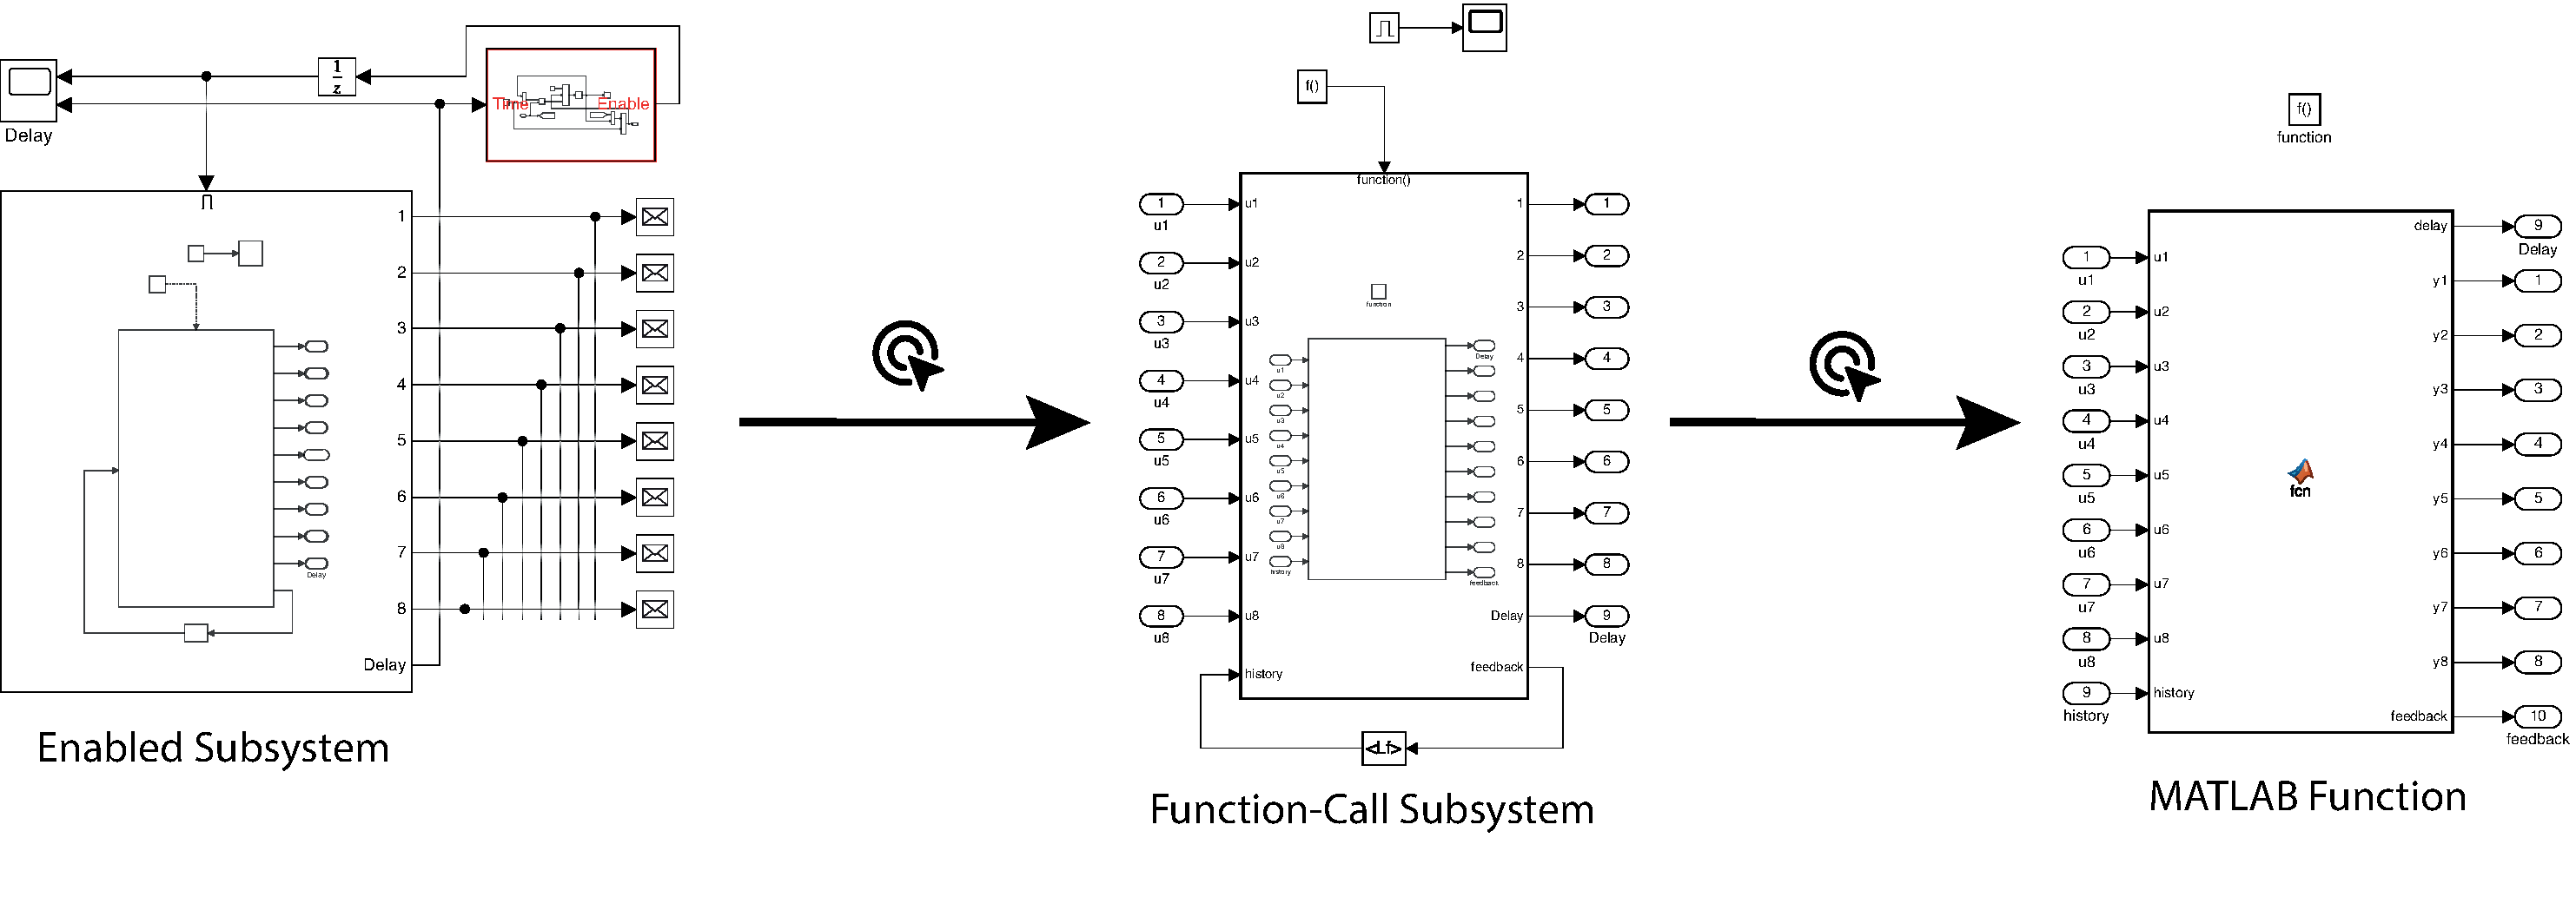
\includegraphics[width=1\textwidth]{functionCaller.pdf}
  \caption{Blocchi inerenti alla funzione di controllo}
  \label{fig:blocchicontrollo}
\end{figure}
\begin{figure}[H]
\center
  
\includegraphics[width=0.2\textwidth]{message.pdf}
  \caption{Il blocco Message Send}
  \label{fig:messagesend}
\end{figure}
\newpage

\textbf{Il timer realizzato:} anche questo componente è in realtà un sottosistema, ovvero, in un blocco \textbf{Subsystem\cite{subsystem}} è stato realizzato un meccanismo per inviare in uscita il numero 1 allo scadere di un timer. Prima di entrare nel merito di quanto creato, è bene notare che l’uscita non controlla direttamente il trigger del blocco Enabled Subsystem, in precedenza descritto, ma che prima venga ritardata di un secondo grazie a un blocco \textbf{Unit Delay\cite{delay}}. Ciò si è reso necessario per evitare alcuni errori, stabilizzando tale uscita.

È dunque chiaro che il timer in realtà non considera esattamente il tempo inviato in uscita dalla funzione, ma aggiunga ad esso un secondo preventivamente, secondo poi recuperato dall’attesa data da questo blocco.

Cliccando due volte sul sottosistema, si può notare come esso sia alquanto elementare. Sfruttando un contatore e fissando il passo di campionamento ad un secondo, ciò che succede è che ogni secondo tale contatore viene incrementato di 1, e viene confrontato con il valore in ingresso, a cui come precedentemente detto viene sommato 1 secondo. Quando questi due valori sono uguali, ovvero quando la loro differenza è nulla, allora il contatore viene resettato, e viene fornita un’uscita pari ad 1.
\begin{figure}[H]
  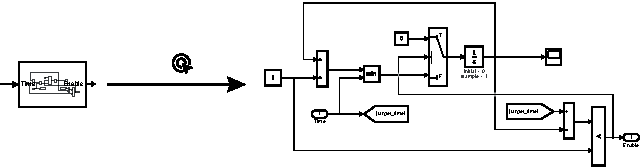
\includegraphics[width=1\textwidth]{temporizzatoreESubsystem.pdf}
  \caption{Il blocco timer realizzato}
  \label{fig:timersub}
\end{figure}
\begin{figure}[H]
\center
  
\includegraphics[width=0.1\textwidth]{1_z.pdf}
  \caption{Il blocco Unit Delay}
  \label{fig:unitdelay}
\end{figure}
\newpage
\textbf{La funzione getTime:} per poter acquisire l'orario della simulazione si è creato, anche questa volta, un oggetto apposito, incapsulato in un blocco \textbf{Simulink Function\cite{simfunc}}. Nello specifico, si è usato un \textbf{Digital Clock\cite{digclock}}, che restituisce un valore numerico che rappresenta il numero di secondi trascorsi dall'avvio della simulazione. Poiché è stato scelto di far durare tale simulazione 86400s, ovvero un giorno, questo numero oscilla fra lo 0 (corrispondente alla mezzanotte) ed 86400, appunto. Collegando tale blocco all'uscita della Simulink Function, si può richiamare la funzione ogni volta che lo si necessita, comprendendo così come far variare i tassi di generazione in base all'ora del giorno.
\begin{figure}[H]
  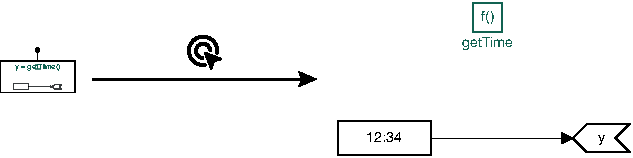
\includegraphics[width=1\textwidth]{digitalClock.pdf}
  \caption{Il blocco Simulink Function per la funzione getTime()}
  \label{fig:gettime}
\end{figure}














\newpage
\section{L'algoritmo di gestione statica dell'incrocio} \label{section: AlgoritmoStatico}
In questa prima fase, come precedentemente accennato, si è voluto modellare il comportamento di un incrocio di questo genere in maniera quanto più possibile fedele alla realtà, per avere un metro di paragone per le successive elaborazioni. Nello specifico, con riferimento alla \textit{figura 1.1}, e come già detto, sono state scelte le direzioni (b), (c), (f), (g), da alternare, concedendo a ciascuna una durata del verde pari a 25 secondi, parametro plausibile se si considera un incrocio grande ed affollato, cosa effettivamente vera, viste le circa 17600 macchine giornaliere.

L’algoritmo implementato è il seguente.

\begin{lstlisting}[language=Matlab,label=static-algorithm,caption= Algoritmo di gestione statica del singolo incrocio]
function [delay, y1, y2, y3, y4, y5, y6, y7, y8, current] = fcn(previous)

GreenTime = 25;
% Current e previous indicano a quale strada si sta dando / si è dato il verde 
current = zeros([1 4]);
next = 1; %Elemento del vettore a cui dare il verde
for i = 1 : 1 : 4
if previous(i) == 1
next = mod(i, 4) + 1;
end
end
current(next) = 1;
%Risultato
U = ([0 0; 0 0; 0 0; 0 0]);
U(next, 1) = 1;
U(next, 2) = 1;
delay = GreenTime; y1 = U(1, 1); y2 = U(1, 2); y3 = U(2, 1); y4 = U(2, 2); y5 = U(3, 1); y6 = U(3, 2); y7 = U(4, 1); y8 = U(4, 2);
%Assegnazione delle uscite

end
\end{lstlisting}
\newpage
La funzione accetta in input \textit{previous}, che è un array di quattro elementi (uno per ogni braccio), nel quale l’unico elemento posto ad uno è quello inerente al braccio che ha ricevuto il verde quando lo script è stato chiamato l’ultima volta. Tutti gli altri valori sono pari a zero. È dunque chiaro che in realtà il vettore in questione si comporta come un canale di feedback, in cui ogni elemento è un flag, e serve per gestire la turnazione.

Come è facile notare, infatti, all’interno dello script viene inizializzato un nuovo array, \textit{current}, sempre di quattro elementi. Si valuta poi quale è stato l’ultimo braccio a cui si è concesso il verde, mediante un \textit{ciclo for}, e si fa scattare il semaforo successivo.

Alla successiva chiamata l’attuale array \textit{current} diventerà a tutti gli effetti il relativo \textit{previous}.

È anche da notare, che oltre alle otto uscite (una per ogni corsia), che in realtà in questo caso statico sono sempre accoppiate (ecco il perché di un vettore \textit{previous} di soli quattro elementi), la funzione manda in output anche il \textit{delay}, ovvero l’intervallo di tempo nel quale le macchine delle strade a cui è stato concesso il verde possono fluire liberamente. Tale \textit{delay} viene poi inviato direttamente al timer, che provvederà a richiamare la funzione alla sua scadenza.

Ogni uscita è poi collegata all’Entity Gate della rispettiva corsia, che, ricevendo 0 si chiude (o resta chiuso), ricevendo 1 permette invece ai veicoli di occupare l’incrocio.
\newpage
\section{Analisi dei risultati}
Si analizzano dunque qui i risultati di questa gestione, utili poi per un confronto con l’algoritmo di ottimizzazione oggetto di questa tesi. In particolare, i grafici che seguono sono ottenuti con una simulazione in cui i parametri $\mu$ per ogni corsia sono i seguenti. Tali grafici, inoltre, si riferiscono alla prima corsia (corsia di sinistra del braccio ovest), dunque al primo parametro di questo vettore.

\begin{center}
	[33.7997   32.4750   23.2955   33.1698   29.9311   24.1165   31.6948   28.4784]
\end{center}

Come si può notare dalla \textit{figura \ref{fig:AutoInCodaStatico}}, riferita al numero di auto in coda in funzione dell’ora del giorno considerata, si ha una sensibile variazione fra il numero di auto in coda durante le ore notturne e quello durante le ore diurne, come era lecito aspettarsi visti i tassi di generazione variabili. È interessante notare come il più alto numero di auto in coda sia 8, con una situazione tende ad assestarsi ad un valore leggermente inferiore. È anche importante considerare che, nonostante i tempi di inter-arrivo notturni siano estremamente elevati, come specificato in precedenza, comunque durante la notte tendano ad accodarsi alcune macchine, fino a un massimo di 5.

Questa è una delle spiegazioni per cui nelle grandi città nelle ore meno affollate molti semafori vengono spenti. Come sarà chiaro più avanti, tuttavia, con un algoritmo di gestione dinamica dell’incrocio, il problema dell’accodamento viene risolto, seppur mantenendo acceso l’apparato semaforico, contribuendo alla sicurezza dei guidatori anche a tarda sera.

La \textit{figura \ref{fig:TempoDiAttesaStatico}} rappresenta invece il tempo medio di attesa delle auto nella corsia considerata, sempre in funzione dell’ora del giorno. Sebbene il tempo concesso a queste auto per defluire sia alquanto importante (ben 25 secondi), si nota come l’attesa tocchi un picco di quasi 95 secondi, in corrispondenza dell’ora di punta, per poi decrescere, seppur di poco. È altresì fondamentale considerare che, proprio per la mancanza di distinzione nel tempo concesso alla luce verde per ciascuna corsia, anche di notte, con un bassissimo affollamento, si assiste ad un’attesa media di più di 35 secondi.

Appare dunque chiaro come siano ampi i margini di miglioramento, sia per quanto riguarda il numero massimo di auto in coda, che, soprattutto, per quanto concerne i tempi medi di attesa, e nel secondo capitolo di questa trattazione saranno analizzati vari metodi per ottimizzare questi due parametri.
\begin{center}
	\begin{figure}[H]
  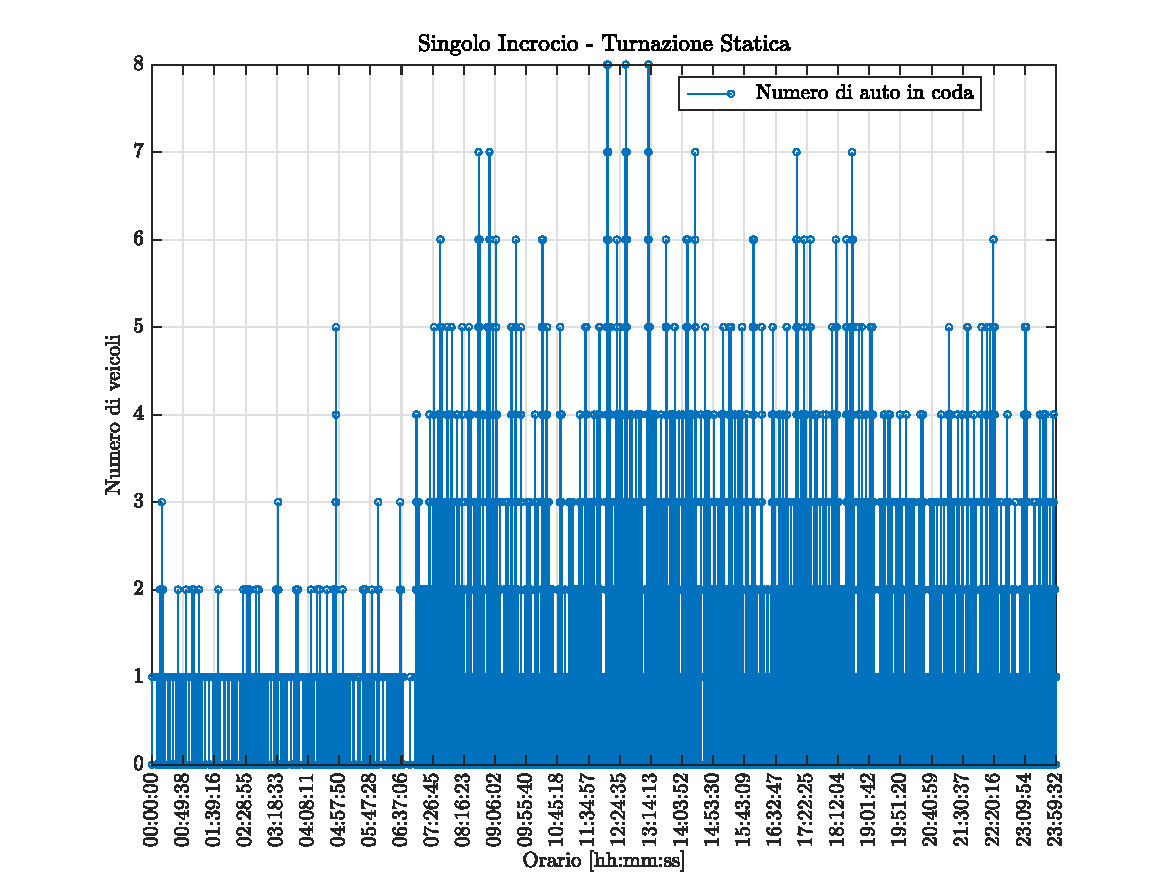
\includegraphics[width=0.90\textwidth]{AutoInCodaStatico.pdf}
  \caption{Numero di auto in coda per una singola corsia}
  \label{fig:AutoInCodaStatico}
\end{figure}
\begin{figure}[H]
  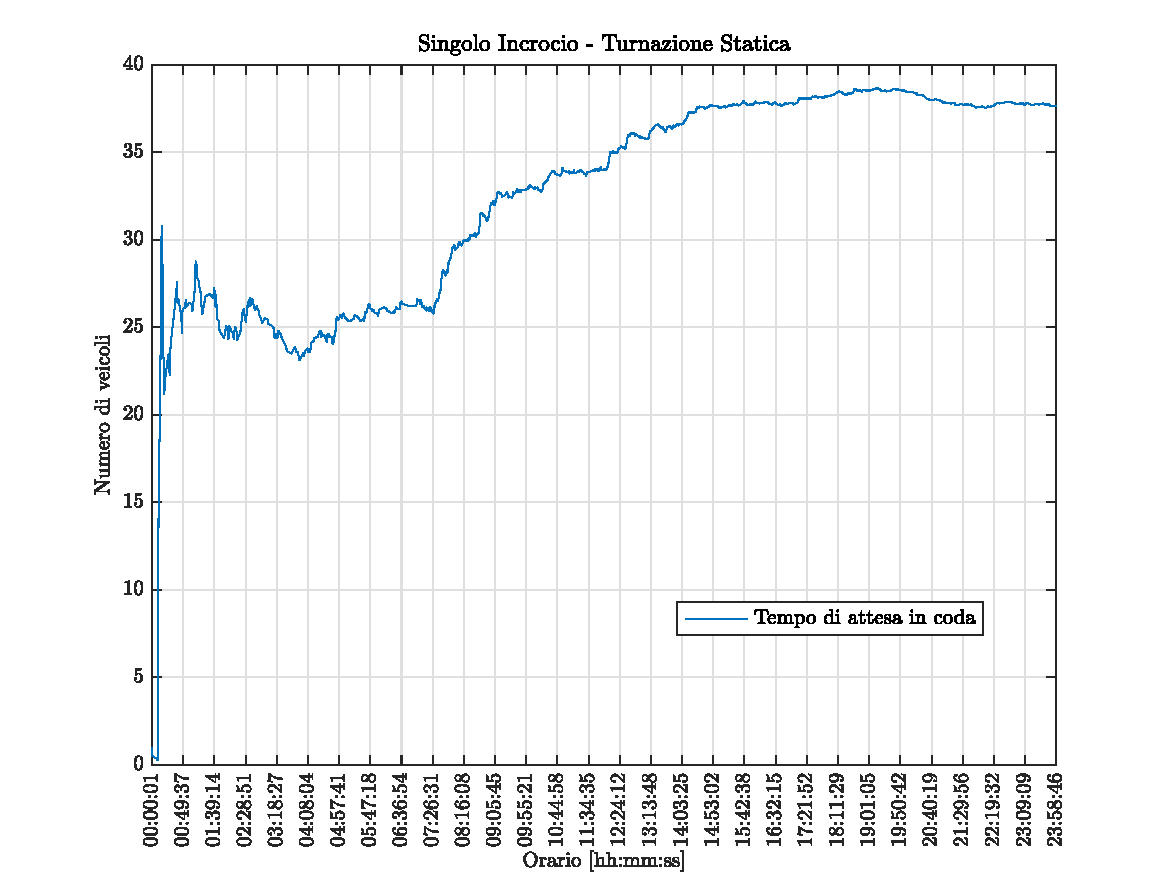
\includegraphics[width=0.90\textwidth]{TempoDiAttesaStatico.pdf}
  \caption{Tempi di attesa medi per una singola corsia in funzione dell'orario considerato}
  \label{fig:TempoDiAttesaStatico}
\end{figure}
\end{center}
\section{Tabella riassuntiva dei risultati con valori variabili del parametro $\mu$}

Nella tabella presente alla seguente pagina sono riportate più esecuzioni dell'algoritmo, sia a fronte dello stesso intervallo relativo al parametro $\mu$, sia per intervalli diversi, per riportare come variano il tempo medio di attesa, il numero di veicoli che attraversano l'incrocio, il numero massimo di veicoli in coda per ogni esecuzione. Tutti questi dati sono inerenti alla singola corsia analizzata, che cambia di esecuzione in esecuzione, come è facile comprendere. 

Nello specifico si può notare come nella prima simulazione, con tassi di generazione elevati (mediamente all'ora di pranzo il tempo di arrivo fra una macchina e l'altra è minore di 10 secondi) si accodi un numero di macchine esagerato nella corsia presa in considerazione. La simulazione è stata infatti portata al limite in questo modo, ed è ovvio che un congestionamento di questo genere è alquanto raro, sebbene non inverosimile; l'obiettivo è stato quello di rendere il lettore consapevole del legame fra il parametro $\mu$ e tutti gli altri valori relativi alla simulazione stessa. Nel capitolo successivo si confronteranno vari scenari, e sarà più immediato capire come, a parità di $\mu$, qualsiasi sia il suo valore, un algoritmo di gestione dinamica è sicuramente più performante.
Risulta anche importante considerare che, a fronte di un sensibile calo del numero di automobili che attraversano l'incrocio, se è vero che cala anche il numero massimo di auto in coda, i tempi di attesa medi restano comunque molto elevati. Sempre al di sopra dei 35 secondi, assolutamente spropositati rispetto a quelli ottenuti con l'algoritmo che verrà proposto nel capitolo successivo.


\begin{table}[H]
\centering
\begin{tabular}{|C{2cm}|c|C{2.25cm}|C{2.25cm}|C{2.25cm}|C{2.25cm}|}
  \hline
  \multicolumn{6}{|c|}{\large Prima simulazione} \\\hline\hline
  \multicolumn{2}{|c|}{\textbf{Intervallo}} &
  \multicolumn{2}{C{5cm}|}{\textbf{Stima tempo interarrivo con minimo $\mu$}} &
  \multicolumn{2}{C{5cm}|}{\textbf{Stima tempo interarrivo con massimo $\mu$}} \\\hline
  \multicolumn{2}{|c|}{$[23, 28]$} &
  \multicolumn{2}{c|}{15.94 secondi} &
  \multicolumn{2}{c|}{19.41 secondi} \\\hline
  \multicolumn{6}{|c|}{\textit{Corsia: Ovest - Dritto/Destra}} \\\hline
  \textbf{\footnotesize Esecuzione} & 
  \textbf{\footnotesize $\mu$} & 
  \textbf{\footnotesize Tempo di arrivo medio} & 
  \textbf{\footnotesize Numero di auto totale} & 
  \textbf{\footnotesize Max numero auto in coda} & 
  \textbf{\footnotesize Tempo di attesa medio} \\\hline
  1 & 
  23.4080 & 
  $16.25s$ & 
  3143 &
  39 &
  $112.61s$ \\\hline
  2 & 
  24.8866 & 
  $17.25s$ & 
  2888 &
  23 &
  $67.03s$ \\\hline
  3 & 
  26.2806 & 
  $18.22s$ & 
  2809 &
  21 &
  $60.08s$ \\\hline
  \multicolumn{6}{c}{}\\\hline
  \multicolumn{6}{|c|}{\large Seconda simulazione} \\\hline\hline
  \multicolumn{2}{|c|}{\textbf{Intervallo}} &
  \multicolumn{2}{C{5cm}|}{\textbf{Stima tempo interarrivo con minimo $\mu$}} &
  \multicolumn{2}{C{5cm}|}{\textbf{Stima tempo interarrivo con massimo $\mu$}} \\\hline
  \multicolumn{2}{|c|}{$[28, 33]$} &
  \multicolumn{2}{c|}{19.41 secondi} &
  \multicolumn{2}{c|}{22.87 secondi} \\\hline
  \multicolumn{6}{|c|}{\textit{Corsia: Nord - Dritto/Destra}} \\\hline
  \textbf{\footnotesize Esecuzione} & 
  \textbf{\footnotesize $\mu$} & 
  \textbf{\footnotesize Tempo di arrivo medio} & 
  \textbf{\footnotesize Numero di auto totale} & 
  \textbf{\footnotesize Max numero auto in coda} & 
  \textbf{\footnotesize Tempo di attesa medio} \\\hline
  1 & 
  32.0241 & 
  $22.20s$ & 
  2314 &
  12 &
  $39.54s$ \\\hline
  2 & 
  30.4146 & 
  $21.08s$ & 
  2381 &
  13 &
  $43.12s$ \\\hline
  3 & 
  28.5156 & 
  $19.77s$ & 
  2553 &
  13 &
  $45.11s$ \\\hline
  \multicolumn{6}{c}{}\\\hline
  \multicolumn{6}{|c|}{\large Terza simulazione} \\\hline\hline
  \multicolumn{2}{|c|}{\textbf{Intervallo}} &
  \multicolumn{2}{C{5cm}|}{\textbf{Stima tempo interarrivo con minimo $\mu$}} &
  \multicolumn{2}{C{5cm}|}{\textbf{Stima tempo interarrivo con massimo $\mu$}} \\\hline
  \multicolumn{2}{|c|}{$[33, 38]$} &
  \multicolumn{2}{c|}{22.87 secondi} &
  \multicolumn{2}{c|}{26.34 secondi} \\\hline
  \multicolumn{6}{|c|}{\textit{Corsia: Sud - Sinistra}} \\\hline
  \textbf{\footnotesize Esecuzione} & 
  \textbf{\footnotesize $\mu$} & 
  \textbf{\footnotesize Tempo di arrivo medio} & 
  \textbf{\footnotesize Numero di auto totale} & 
  \textbf{\footnotesize Max numero auto in coda} & 
  \textbf{\footnotesize Tempo di attesa medio} \\\hline
  1 & 
  37.3261 & 
  $25.87s$ & 
  1960 &
  9 &
  $35.55s$ \\\hline
  2 & 
  33.6499 & 
  $23.32s$ & 
  2206 &
  9 &
  $38.69s$ \\\hline
  3 & 
  36.4679 & 
  $25.28s$ & 
  1923 &
  7 &
  $35.61s$ \\\hline
\end{tabular}
\caption{Esecuzioni dell'algoritmo di gestione statica al variare di $\mu$}
\label{table:tabellaconfrontostatico}
\end{table}








%inizio capitolo 2
\chapter{Algoritmo di gestione dinamica applicato ad un singolo incrocio}

In questo capitolo si vuole analizzare il comportamento dello stesso incrocio visto in precedenza con un algoritmo di gestione ottimizzata, che conti il numero di auto in ciascuna corsia e in base a questo e ad altri parametri conceda il verde per un numero di secondi variabile. È da precisare che l’algoritmo utilizzato si basa su quello proposto da \textit{Maram Bani Younes e Azzedine Boukerche}\cite{itlc}, tuttavia sono state effettuate alcune importanti modifiche, che verranno analizzate nel corso della trattazione. 

Si è previsto,  oltre che un raffronto fra l'algoritmo di gestione statica e quello sviluppato in autonomia, modificando quanto proposto dai due ingegneri, anche un meccanismo per valutare l'efficacia di queste modifiche, confrontando il nuovo codice con una implementazione di quello presente nella pubblicazione citata. Tutti i confronti, con i relativi grafici e le relative conclusioni, verranno presentati alla fine di questo capitolo, dopo aver descritto nel dettaglio tutti gli aspetti relativi alle modifiche apportate al modello e ai meccanismi implementativi adottati.


Per quanto riguarda lo pseudocodice progettato dai due ingegneri, è disponivile alla seguente pagina.
\newpage
\begin{lstlisting}[language=C,label=pseudocode,caption=Pseudocodice di gestione dinamica di un incrocio]
while d_i di una qualsiasi corsia > 0 do
{
	
	sia j la corsia con il maggior numero di macchine;
	siano i_1 e i_2 le due corsie complementari;
		if (d_i_1 > d_i_2)
		{
			schedula j,i_1;
			d_i_1 = 0;
			t_i_1 = 0;
		}
		
		else
		{
			schedula j,i_2;
			d_i_2 = 0;
			t_i_2 = 0;
		}
		d_j = 0;
		t_j = 0;
	
}   
\end{lstlisting}
\newpage
\section{Breve spiegazione dell'algoritmo originale}
La proposta di \textit{Maram Bani Younes e Azzedine Boukerche} si basa sulla definizione di alcuni parametri, il primo dei quali è la così detta \textit{Ready Area}. Tale area è sostanzialmente il range entro il quale le macchine si possono considerare in coda per l’incrocio: si individua, per ogni semaforo della giunzione, una distanza massima, di solito corrispondente alla portata del dispositivo di rilevazione in termini di veicoli, oltre la quale le vetture non vengono più conteggiate. 

Il dispositivo in questione può essere rappresentato da una semplice telecamera che, mediante meccanismi tipici della Computer Vision, utilizzando API quali Google Vision\cite{google_vision} o OpenCV\cite{open_CV}, riesca ad individuare la variabile principale su cui si basa l’algoritmo: il numero di auto in coda per ciascuna corsia. L’implementazione hardware di questo sistema, tuttavia, non è oggetto di questa tesi e dunque non ci si dilungherà oltre nella sua spiegazione.

Il tempo concesso alle corsie prescelte (durata della luce verde) è poi dinamico, e viene calcolato sulla base della seguente formula: 

\begin{equation} \label{eq:}
  T = \theta + \frac{F_d}{S_{tf}}
\end{equation}

Il parametro $\theta$ è una costante, e rappresenta il tempo che mediamente è necessario alla prima macchina per partire, mentre $F_d$ è la distanza del veicolo più lontano dal semaforo (sempre interno alla \textit{Ready Area} ). In ultimo, $S_{tf}$ è la velocità media del flusso di auto nell’intersezione. Come è ovvio notare, sia $\theta$ che $S_{tf}$ sono ottenuti mediante delle stime, non essendo misurabili prima della effettiva esecuzione dell’algoritmo. 

Una proposta alternativa, certamente più efficiente ma anche meno facile da implementare, è quella di permettere alle automobili di comunicare fra loro e con il semaforo dati quali la $F_d$ (distanza), nonché la loro velocità media. Certamente in questo modo si renderebbe l’esecuzione dello script più veritiera ed affidabile, ed in futuro, grazie agli sforzi delle case automobilistiche, probabilmente tutto ciò sarà possibile.

Altri parametri da considerare sono $d_i$ che rappresenta il numero di automobili in coda nella corsia i-esima e $t_i$, tempo richiesto a tutti i veicoli della corsia i-esima (all’interno della \textit{Ready Area}) per lasciare l’intersezione.

\textbf{Il funzionamento dell’algoritmo è dunque il seguente:} si individua la corsia più affollata fra quella che presentano almeno un’automobile, e contestualmente si rintracciano le due corsie compatibili con essa, così come spiegato nel \textit{Capitolo \ref{capitolo1}} e come si può notare nella \textit{figura \ref{dirCompatibili}}.

A questo punto, fra queste due candidate si sceglie ancora la più affollata; in questo modo non solo si va a concedere il verde alla strada con più automobili, ma si cerca anche di ottimizzare la scelta della sua complementare, che non resta statica (come invece è nell’algoritmo utilizzato nel capitolo precedente), ma diventa dinamica ed intelligente. Successivamente l’algoritmo prevede di calcolare il tempo \textit{T}, concedendolo alla luce verde delle due corsie, e di azzerare le variabili $d_i, d_j$ e $t_i, t_j$ relative, in quanto si prevede che dopo T secondi le corsie in questione presentino un numero di veicoli pari a zero.
\newpage
\section{Le modifiche apportate}
Sono molteplici le modifiche apportate all’algoritmo proposto, alcune delle quali a puro scopo implementativo, altre come migliorie.

In primo luogo, si è preferito non considerare una \textit{Ready Area} per non dover dare alle code di \textit{Simulink} un massimo numero di entità (veicoli) da contenere, questo per effettuare più simulazioni variando i tassi di generazione, verificando il comportamento del modello anche in condizioni esageratamente negative, con code anche molto affollate (più di 50 automobili). 

Il concetto della \textit{Ready Area}, tuttavia, non è stato abbandonato del tutto, ma è stato piuttosto migliorato: si è deciso di concedere un tempo minimo ed un tempo massimo alla durata del verde per ciascuna corsia. Il tempo minimo serve perché, anche con una sola macchina in coda, si è voluto stabilizzare la situazione, che altrimenti si sarebbe tradotta in un passaggio troppo repentino dal verde al rosso. Per quanto concerne il tempo massimo, questo è diretta espressione della \textit{Ready Area}: invece che considerare un massimo numero di veicoli, si considera che, indipendentemente da questo numero, il verde non può durare più di un certo valore, questo per evitare tempi di attesa troppo lunghi nelle corsie meno affollate, ma comunque in cui sono presenti veicoli. 

Il tempo concesso alla luce verde, poi, viene calcolato tenendo conto della distribuzione uniforme che governa gli \textit{Entity Server}, precedentemente descritta, assegnando ad ogni macchina un valore pari al valore medio della distribuzione (in questa simulazione pari a $5s$), ed ottenendo il tempo complessivo moltiplicando questo valore per il numero di veicoli in coda. A questo punto, se il numero ottenuto è inferiore al tempo minimo, esso si scarta, e si prende in considerazione proprio quel minimo, viceversa se supera il tempo massimo è questo ad essere tenuto in considerazione e ad essere concesso. Pertanto, poiché non è detto che le code a cui viene dato il via libera si svuotino, non si va ad azzerare i contatori relativi, ma semplicemente all'esecuzione successiva della funzione questi sono aggiornati con i nuovi dati rilevati, ottenuti dalle code stesse.

Inoltre, è stata individuata una grande lacuna nell’algoritmo oggetto della pubblicazione citata: l’assenza di un meccanismo di gestione della \textit{starvation}. 

Considerando esclusivamente il \textit{codice \ref{pseudocode}}, infatti, si nota che se in una strada continuano a confluire veicoli più velocemente che nelle altre, a questa sarà sempre concesso il verde. Questo comportamento da un lato è positivo perché si va a decongestionare tale corsia, ma è ovviamente improponibile, in quanto potrebbe paradossalmente capitare che un semaforo resti rosso per ore ed ore, e che una persona sia costretta ad attendere un tempo esagerato prima di passare, perché la sua strada è meno affollata.

È stato scelto dunque di implementare un meccanismo di gestione della \textit{starvation} mediante un algoritmo \textit{LRU} (Least Recently Used) opportunamente modificato. Ad ogni corsia è associato un contatore, ed ogni qual volta ad una strada viene concesso il verde, il suo contatore viene azzerato, mentre quello delle altre si incrementa del numero di secondi per cui è stato concesso il verde alla corsia suddetta. In questo modo, quando un contatore raggiunge un valore limite (liberamente impostabile), la relativa strada ottiene priorità massima, e l’algoritmo viene applicato in maniera identica (calcolo del tempo del verde e selezione della complementare) come se essa fosse quella più affollata. In particolare il tempo massimo di attesa prima che scatti la starvation è stato impostato a 5 minuti.

È anche da notare che sono stati apportati alcuni minimi cambiamenti al modello: le code sono state collegate agli ingressi del blocco contenente la funzione da eseguire, comunicando ad essa il numero di veicoli presenti, ed il canale di \textit{feedback} è stato utilizzato per implementare il meccanismo della gestione della \textit{starvation}, e non per conoscere a quale semaforo è stato concesso il verde nell’esecuzione precedente, informazione ora inutile. Non è stato variato altro, se non, ovviamente, il codice nel blocco \textit{Matlab Function}, quindi non si ravvisa la necessità di approfondire nuovamente la necessità di descrivere nei dettagli nuovamente l'intero modello, il cui schema è comunque presente alla pagina seguente, seguito dal codice che lo governa.

\begin{figure}[H]
  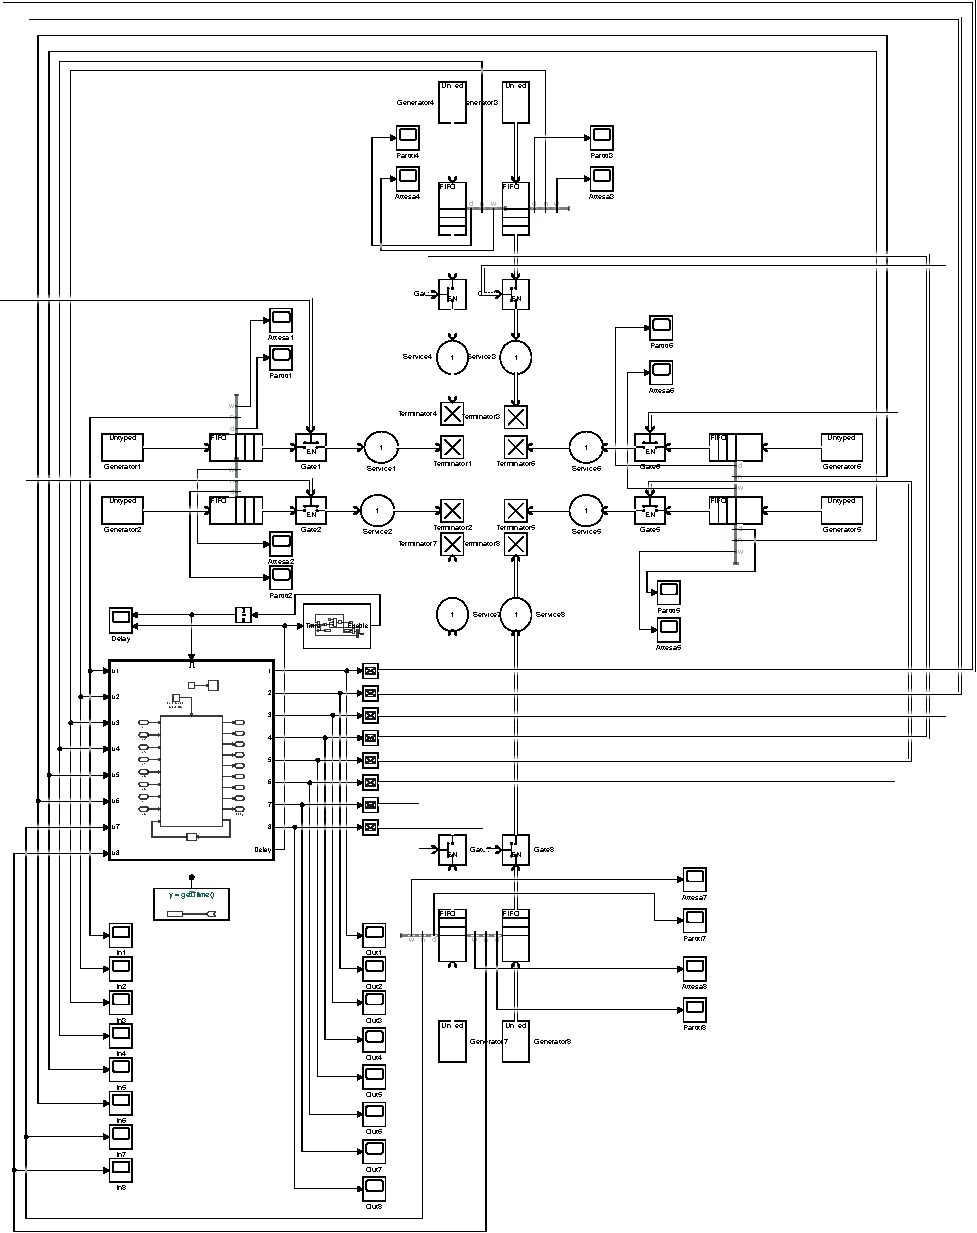
\includegraphics[width=1\textwidth]{SingoloIncrocioAlgoritmo.pdf}
  \caption{Modello di un incrocio a raso a quattro bracci in Simulink e SimEvents, gestione dinamica}
  \label{fig:modellosingoloincrocioalgoritmo}
\end{figure}
\newpage

\begin{lstlisting}[language=Matlab,label=key,caption=Implementazione dell'algoritmo di gestione dinamica di un singolo incrocio]
function [delay, y1, y2, y3, y4, y5, y6, y7, y8, feedback] = fcn(u1, u2, u3, u4, u5, u6, u7, u8, history)


% VARIABILI DI USCITA
% Prima attesa, prima dell'esecuzione dell'algoritmo la prima volta
delay = 1; 
y1 = 0; 
y2 = 0; 
y3 = 0; 
y4 = 0; 
y5 = 0; 
y6 = 0; 
y7 = 0;
y8 = 0;
feedback = zeros([4 2]);
 
% Numero di veicoli per ogni direzione
M = ([u1 u2; u3 u4; u5 u6; u7 u8;]);
 
% Tempo medio per fluire per ogni macchina
Tv = 5;
 
% Massimo tempo del verde
MaxGreen = 60;
 
% Minimo tempo del verde
MinGreen = 10;
 
% Controllo sulla starvation (LRU). Tempo di attesa massimo: 5 minuti
starvation = 300;
 
% Cerco il massimo
[R, C] = size(M);
iMax = 1;
jMax = 1;
vMax = M(1, 1);
 
%Usato per la starvation, interrompe la ricerca
flag = 0;
 
for i = 1 : 1 : R
    for j = 1 : 1 : C
        
        if M(i, j) > 0 && history(i, j) > starvation
            vMax = M(i, j);
            iMax = i;
            jMax = j;
            flag = 1;
            break;
        end
 
        if M(i, j) > vMax
            vMax = M(i, j);
            iMax = i;
            jMax = j;
        end
       
    end
    
    if flag == 1
        break;
    end
end
 
 
% Cerco i possibili candidati
[c1_i, c1_j, c2_i, c2_j] = getCandidates(iMax, jMax);
 
%Scelgo tra i candidati
if M(c1_i, c1_j) > M(c2_i, c2_j) 
    iCan = c1_i;
    jCan = c1_j;
else
    iCan = c2_i;
    jCan = c2_j;
end
 
delay = vMax*Tv;
 
if vMax*Tv > MaxGreen
        delay = MaxGreen;
elseif vMax*Tv < MinGreen
        delay = MinGreen;
end
    
%Risultato
U = ([0 0; 0 0; 0 0; 0 0]);
 
U(iMax, jMax) = 1;
U(iCan, jCan) = 1;
     
history( : ) = history( : ) + delay;
    
history(iMax, jMax) = 0;
history(iCan, jCan) = 0;

%Output 
y1 = U(1, 1); y2 = U(1, 2); y3 = U(2, 1); y4 = U(2, 2); y5 = U(3, 1); y6 = U(3, 2); y7 = U(4, 1); y8 = U(4, 2); feedback(:) = history(:);
end
    
\end{lstlisting}
\newpage
\section{Spiegazione del codice implementato}
In primo luogo vengono inizializzate le variabili in uscita della funzione, corrispondenti al valore di trigger degli otto entity gate rappresentanti le varie corsie. Di default questi valori sono posti a 0 (semaforo rosso). In input si accetta il numero di veicoli presenti in ogni coda nell'istante in cui la funzione viene richiamata, nonché il vettore \textit{history}, usato per gestire la starvation, il cui significato sarà chiaro più avanti.

I due \textit{cicli for} annidati servono ad individuare la strada con il numero di veicoli più elevato, purché non si verifichi il caso di \textit{starvation}. Tale strada (individuata da due indici, \textit{i} e \textit{j} all’interno della matrice \textit{M}, matrice che organizza gli otto input indipendenti), viene poi data in pasto alla funzione \textit{getCandidates}, il cui codice è alla pagina seguente e che restituisce gli indici relativi alla matrice M che individuano le due strade che possono essere scelte assieme alla principale. A questo punto fra le due corsie complementari candidate viene scelta, come già detto, quella più affollata. Viene calcolato il tempo da concedere al verde in funzione del numero di veicoli della strada scelta come principale, e vengono effettuati i controlli con il tempo minimo ed il tempo massimo, precedentemente dichiarati come costanti.

Successivamente, ogni elemento del vettore \textit{History}, il quale contiene i contatori inerenti all’algoritmo \textit{LRU} per ogni corsia, viene incrementato del tempo stabilito, azzerando poi gli elementi corrispondenti alle corsie a cui si sta concedendo il verde.

In output viene inviato \textit{1} agli \textit{Entity Gate} che devono aprirsi, corrispondenti alle strade individuate, e \textit{0} a tutti gli altri. 

Oltre a queste informazioni rappresenta un output anche il \textit{delay}, ovvero proprio il tempo concesso, che viene inviato al timer descritto nel \textit{capitolo \ref{capitolo1}}, che richiamerà la funzione allo scadere dello stesso.
\newpage
\begin{lstlisting}[language=Matlab,label=key,caption=Scelta delle due strade complementari a quella selezionata come principale]
    function [i1, j1, i2, j2] = getCandidates(i, j)
    % Direzioni accoppiate (8x4)
    % Per ciascuna direzione scelta, ci sono 2 possibili direzioni
    % complementari
    % D = {[1 2; 3 1] [1 1; 3 2]; [4 1; 2 2] [2 1; 4 2]; [3 2; 1 1] [3 1; 1 2]; [4 2; 2 1] [4 1; 2 2]};
    
    i1 = 0;
    i2 = 0;
    j1 = 0;
    j2 = 0;
    
    if i==1 && j ==1
        i1 = 1;
        j1 = 2;
        i2 = 3;
        j2 = 1;
    elseif i==1 && j==2
       i1 = 1;
       j1 = 1;
       i2 = 3;
       j2 = 2;
    elseif i==2 && j==1
       i1 = 4;
       j1 = 1;
       i2 = 2;
       j2 = 2;
    elseif i==2 && j==2
       i1 = 2;
       j1 = 1;
       i2 = 4;
       j2 = 2;
    elseif i==3 && j==1
       i1 = 3;
       j1 = 2;
       i2 = 1;
       j2 = 1;
    elseif i==3 && j==2
       i1 = 3;
       j1 = 1;
       i2 = 1;
       j2 = 2;
    elseif i==4 && j==1
       i1 = 4;
       j1 = 2;
       i2 = 2;
       j2 = 1;
    elseif i==4 && j==2
       i1 = 4;
       j1 = 1;
       i2 = 2;
       j2 = 2;
    end
            
        
end
\end{lstlisting}

È da sottolineare che questo codice funziona fintanto che gli ingressi non vengono variati: se si dovesse collegare una strada ad un ingresso diverso da quello previsto ed utilizzato nella simulazione chiaramente l’intero algoritmo non sarebbe più affidabile. L'autore di questa tesi è consapevole che esistono metodi più eleganti ed ottimizzati rispetto a questa sequenza di \textit{if} ed \textit{elseif} per ottenere il medesimo scopo, tuttavia si è reso necessario procedere in questo modo per lo scarso supporto del linguaggio \textit{Matlab} a tali meccanismi, come, per esempio, gli \textit{switch - case}. In questo modo, inoltre, il codice risulta particolarmente leggibile e facile da comprendere.
\newline

Le differenze con un normale algoritmo di gestione di una giunzione, come quello proposto nel \textit{capitolo \ref{capitolo1}} sono quindi evidenti: in primo luogo non si segue una turnazione statica per quanto riguarda la concessione del verde, seguendo invece un meccanismo di priorità: ci si chiede infatti quale sia la strada che necessita del verde in quell'istante, più delle altre, e glielo si concede. Inoltre anche il tempo per cui questo verde è concesso è variabile: si ipotizzi per esempio di analizzare l'incrocio durante le ore notturne, non avrebbe senso concedere il verde per un numero di secondi elevato quando in coda è presente una sola macchina, si tratterebbe di una perdita di tempo, tradotta in un maggior consumo di carburante ed un maggiore stress per gli automobilisti delle altre corsie, costretti ad attendere perché viene concesso il verde ad una strada praticamente vuota. Viceversa è ovvio che durante il giorno, per una strada affollata, la durata della luce verde deve essere sufficiente da garantire che un buon numero delle macchine in coda defluisca.
\newpage

\section{Il modello per confrontare le diverse gestioni del singolo incrocio}

I benefici esposti, ovviamente, devono trovare riscontro in un confronto imparziale ed assolutamente valido fra i modelli presentati, affinché a partire dai medesimi dati in input (le automobili generate), e con gli stessi parametri (tasso di generazione, tempo di servizio interno agli \textit{Entity Server}) essi gestiscano l'incrocio secondo la propria logica. Si è scelto, pertanto, di creare in un nuovo workspace il modello identificato dalla \textit{figura \ref{fig:gatecontrolcompare}}. Si può notare come al suo interno siano presenti tre blocchi principali, ognuno dei quali è rappresentativo di un algoritmo di gestione. Guardando infatti ai tre blocchi presenti, si comprende subito come questi siano in realtà esattamente i modelli precedentemente descritti. Il primo, quello più in alto a sinistra, è quello presentato nel \textit{capitolo \ref{capitolo1}}, relativo ad una gestione statica (\textit{figura \ref{fig: modelloSingoloIncrocio}}). Quello in basso a sinistra invece si riferisce al modello di controllo dinamico, di cui si è parlato in questo capitolo (\textit{figura \ref{fig:modellosingoloincrocioalgoritmo}}), mentre quello in basso a destra è perfettamente identico a quest'ultimo, eccezion fatta per la gestione della starvation, che si è eliminata. Ciò è stato fatto per capire come tale gestione, che comunque resta assolutamente necessaria, interferisca con il normale funzionamento dell'algoritmo stesso.

Nello specifico, in questo terzo modello, si è provveduto semplicemente a commentare la seguente porzione di codice, lasciando tutto il resto invariato.
\newline
\begin{lstlisting}[language=Matlab,label=starvation,caption= Porzione di codice relativa alla gestione della starvation]
    if M(i, j) > 0 && history(i, j) > starvation
            vMax = M(i, j);
            iMax = i;
            jMax = j;
            flag = 1;
            break;
    end
        ...
        ...
        ...
   if flag == 1
        break;
   end
\end{lstlisting}

Gli \textit{Entity Generator}, poi, sono stati collegati a dei blocchi di tipo \textbf{Entity Replicator\cite{entityreplicator}}, in modo tale che appena una entità viene generata in una corsia specifica, questa venga subito inviata ai tre modelli contemporaneamente. In questo modo i tre incroci sono esattamente identici sia per quanto riguarda il numero di entità che devono gestire che per quanto concerne quando queste si presentano, tutto questo per garantire l'assoluta imparzialità delle condizioni, precedentemente citata.
\newline

Dunque il workflow è il seguente: quando una entità viene generata, questa viene inviata a tutti e tre gli incroci, in corrispondenza della stessa corsia e nello stesso istante di tempo. La simulazione parte allo stesso istante per tutti e tutti sono configurati secondo gli stessi parametri. Al termine della simulazione tutti gli incroci producono tre grafici per ogni corsia, relativi al tempo di attesa medio, al numero di macchine totali che hanno attraversato tale strada ed al numero medio di macchine in coda in funzione dell'ora del giorno. Confrontando i grafici di una stessa strada, e facendo questo per ogni strada presente, si ottiene una chiara idea di quale dei tre algoritmi stia funzionando meglio.

\newpage

\begin{figure}[H]
  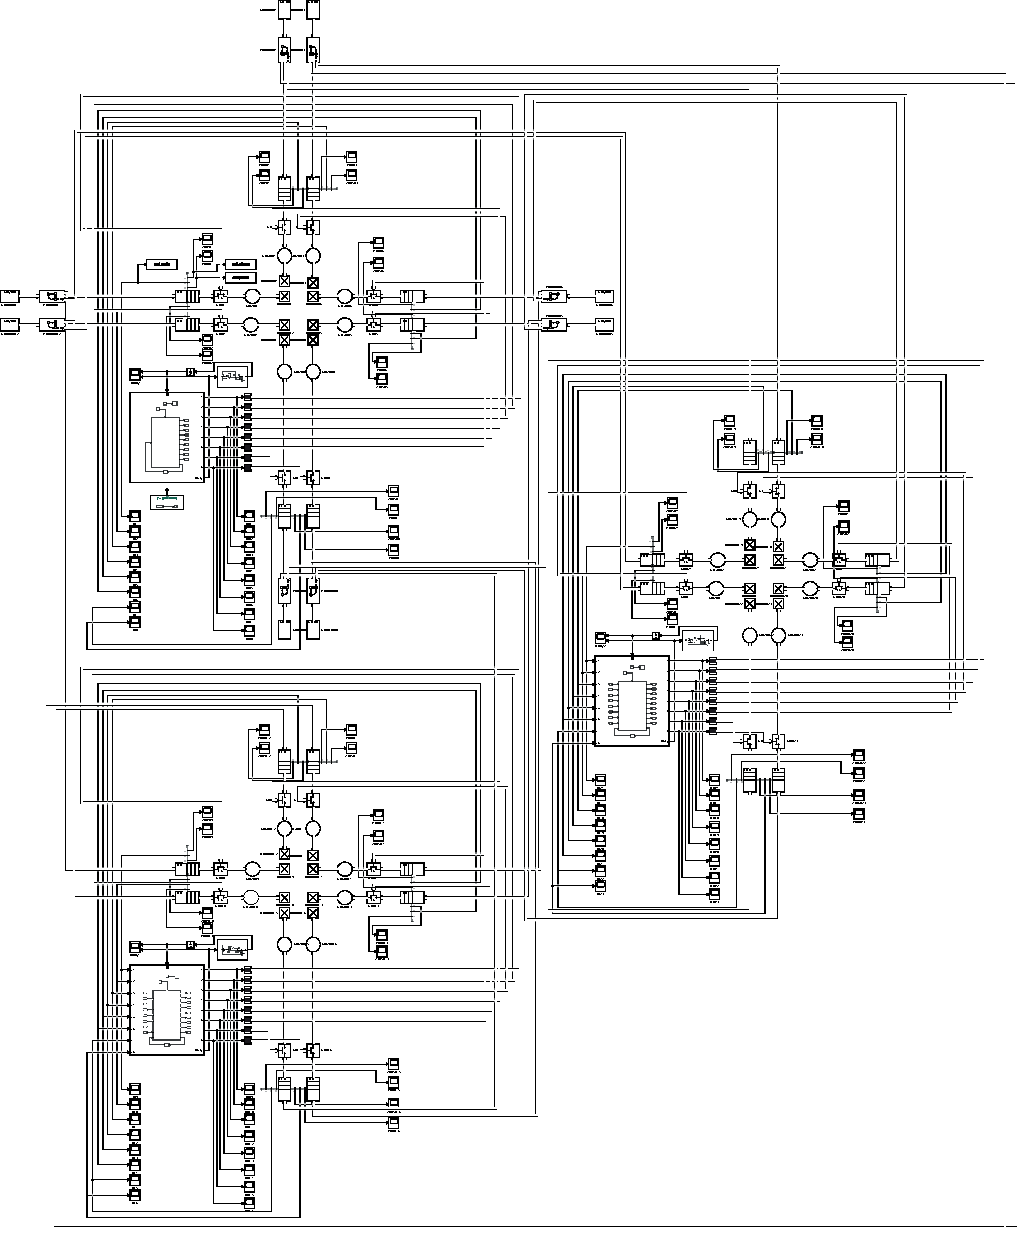
\includegraphics[width=1\textwidth]{GateControlCompare.pdf}
  \caption{Modello per comparare gli algoritmi utilizzati per la gestione di un singolo incrocio}
  \label{fig:gatecontrolcompare}
\end{figure}

\newpage
\section{I risultati ottenuti}
Per le seguenti simulazioni il primo scenario, ovvero il seguente, presenta dei tassi di generazione randomici, esattamente come nel \textit{capitolo \ref{capitolo1}}, con il parametro $\mu$ scelto casualmente, secondo una distribuzione uniforme, fra 23 e 35. Questo per ottenere un numero di automobili sì variabile, ma che sia confrontabile fra le varie strade, con una configurazione dunque che può dirsi bilanciata. Il codice interno agli \textit{Entity Generator} non è dunque stato variato rispetto a quanto presentato nel \textit{codice \ref{mu-definition}}, così come la definizione dei parametri globali (\textit{codice \ref{entity-generator}}). In una configurazione di questo genere sono stati ottenuti i risultati riportati nelle seguenti tabelle, a fronte di questi valori di $\mu$ generati.
\newline

\begin{table}[H]
\centering
\begin{tabular}{|C{2cm}|C{1.65cm}|C{1.65cm}|C{1.65cm}|C{1.65cm}|C{1.65cm}|C{1.65cm}|}
  \hline
  \multicolumn{7}{|c|}{\large Prima simulazione: prime quattro corsie} \\\hline\hline
  \textbf{Intervallo} &
  \multicolumn{3}{C{5.8cm}|}{\textbf{Stima tempo interarrivo con minimo $\mu$}} &
  \multicolumn{3}{C{5.8cm}|}{\textbf{Stima tempo interarrivo con massimo $\mu$}} \\\hline
  $[23, 35]$ &
  \multicolumn{3}{c|}{$15.94s$} &
  \multicolumn{3}{c|}{$24.26$} \\\hline
  \multirow{7}{2cm}{\centering \textit{\footnotesize{Corsia Ovest \newline --- \newline Sinistra}}}
  & \multicolumn{2}{C{3.7cm}|}{\textbf{$\mu$}} 
  & \multicolumn{2}{C{3.7cm}|}{\textbf{\footnotesize{Tempo di arrivo medio}}} 
  & \multicolumn{2}{C{3.7cm}|}{\textbf{\footnotesize{Numero di auto totale}}} \\\cline{2-7}
  & \multicolumn{2}{C{3.7cm}|}{24.1705} 
  & \multicolumn{2}{C{3.7cm}|}{$16.75s$} 
  & \multicolumn{2}{C{3.7cm}|}{2940} \\\cline{2-7}
  & \multicolumn{2}{C{3.7cm}|}{\footnotesize{\textbf{Gestione statica}}} 
  & \multicolumn{2}{C{3.7cm}|}{\footnotesize{\textbf{Gestione dinamica senza starvation}}} 
  & \multicolumn{2}{C{3.7cm}|}{\footnotesize{\textbf{Gestione dinamica con starvation}}} \\\cline{2-7}
  & \scriptsize{Max numero auto in coda}
  & \scriptsize{Tempo di attesa medio}
  & \scriptsize{Max numero auto in coda}
  & \scriptsize{Tempo di attesa medio}
  & \scriptsize{Max numero auto in coda}
  & \scriptsize{Tempo di attesa medio}\\\cline{2-7}
  & 25
  & $59.44s$
  & 11
  & $19.18s$
  & 13
  & $19.07s$\\\hline\hline
    \multirow{7}{2cm}{\centering \textit{\footnotesize{Corsia Ovest \newline --- \newline Dritto/Destra}}}
  & \multicolumn{2}{C{3.7cm}|}{\textbf{$\mu$}} 
  & \multicolumn{2}{C{3.7cm}|}{\textbf{\footnotesize{Tempo di arrivo medio}}} 
  & \multicolumn{2}{C{3.7cm}|}{\textbf{\footnotesize{Numero di auto totale}}} \\\cline{2-7}
  & \multicolumn{2}{C{3.7cm}|}{26.3420} 
  & \multicolumn{2}{C{3.7cm}|}{$18.26s$} 
  & \multicolumn{2}{C{3.7cm}|}{2809} \\\cline{2-7}
  & \multicolumn{2}{C{3.7cm}|}{\footnotesize{\textbf{Gestione statica}}} 
  & \multicolumn{2}{C{3.7cm}|}{\footnotesize{\textbf{Gestione dinamica senza starvation}}} 
  & \multicolumn{2}{C{3.7cm}|}{\footnotesize{\textbf{Gestione dinamica con starvation}}} \\\cline{2-7}
  & \scriptsize{Max numero auto in coda}
  & \scriptsize{Tempo di attesa medio}
  & \scriptsize{Max numero auto in coda}
  & \scriptsize{Tempo di attesa medio}
  & \scriptsize{Max numero auto in coda}
  & \scriptsize{Tempo di attesa medio}\\\cline{2-7}
  & 18
  & $52.61s$
  & 8
  & $17.27s$
  & 10
  & $17.34s$\\\hline\hline
  \multirow{7}{2cm}{\centering \textit{\footnotesize{Corsia Nord \newline --- \newline Sinistra}}}
  & \multicolumn{2}{C{3.7cm}|}{\textbf{$\mu$}} 
  & \multicolumn{2}{C{3.7cm}|}{\textbf{\footnotesize{Tempo di arrivo medio}}} 
  & \multicolumn{2}{C{3.7cm}|}{\textbf{\footnotesize{Numero di auto totale}}} \\\cline{2-7}
  & \multicolumn{2}{C{3.7cm}|}{29.5626} 
  & \multicolumn{2}{C{3.7cm}|}{$20.49s$} 
  & \multicolumn{2}{C{3.7cm}|}{2384} \\\cline{2-7}
  & \multicolumn{2}{C{3.7cm}|}{\footnotesize{\textbf{Gestione statica}}} 
  & \multicolumn{2}{C{3.7cm}|}{\footnotesize{\textbf{Gestione dinamica senza starvation}}} 
  & \multicolumn{2}{C{3.7cm}|}{\footnotesize{\textbf{Gestione dinamica con starvation}}} \\\cline{2-7}
  & \scriptsize{Max numero auto in coda}
  & \scriptsize{Tempo di attesa medio}
  & \scriptsize{Max numero auto in coda}
  & \scriptsize{Tempo di attesa medio}
  & \scriptsize{Max numero auto in coda}
  & \scriptsize{Tempo di attesa medio}\\\cline{2-7}
  & 10
  & $38.86s$
  & 9
  & $24.02s$
  & 10
  & $22.85s$\\\hline\hline
  \multirow{7}{2cm}{\centering \textit{\footnotesize{Corsia Nord \newline --- \newline Dritto/Destra}}}
  & \multicolumn{2}{C{3.7cm}|}{\textbf{$\mu$}} 
  & \multicolumn{2}{C{3.7cm}|}{\textbf{\footnotesize{Tempo di arrivo medio}}} 
  & \multicolumn{2}{C{3.7cm}|}{\textbf{\footnotesize{Numero di auto totale}}} \\\cline{2-7}
  & \multicolumn{2}{C{3.7cm}|}{34.4901} 
  & \multicolumn{2}{C{3.7cm}|}{$23.91s$} 
  & \multicolumn{2}{C{3.7cm}|}{2049} \\\cline{2-7}
  & \multicolumn{2}{C{3.7cm}|}{\footnotesize{\textbf{Gestione statica}}} 
  & \multicolumn{2}{C{3.7cm}|}{\footnotesize{\textbf{Gestione dinamica senza starvation}}} 
  & \multicolumn{2}{C{3.7cm}|}{\footnotesize{\textbf{Gestione dinamica con starvation}}} \\\cline{2-7}
  & \scriptsize{Max numero auto in coda}
  & \scriptsize{Tempo di attesa medio}
  & \scriptsize{Max numero auto in coda}
  & \scriptsize{Tempo di attesa medio}
  & \scriptsize{Max numero auto in coda}
  & \scriptsize{Tempo di attesa medio}\\\cline{2-7}
  & 11
  & $37.12s$
  & 8
  & $21.31s$
  & 7
  & $21.43s$\\\hline
\end{tabular}
\caption{Tabella di comparazione fra algoritmi di gestione del singolo incrocio - prime quattro corsie}
\label{table:keytable}
\end{table}
\newpage

\begin{table}[H]
\centering
\begin{tabular}{|C{2cm}|C{1.65cm}|C{1.65cm}|C{1.65cm}|C{1.65cm}|C{1.65cm}|C{1.65cm}|}
  \hline
  \multicolumn{7}{|c|}{\large Prima simulazione: ultime quattro corsie} \\\hline\hline
  \textbf{Intervallo} &
  \multicolumn{3}{C{5.8cm}|}{\textbf{Stima tempo interarrivo con minimo $\mu$}} &
  \multicolumn{3}{C{5.8cm}|}{\textbf{Stima tempo interarrivo con massimo $\mu$}} \\\hline
  $[23, 35]$ &
  \multicolumn{3}{c|}{$15.94s$} &
  \multicolumn{3}{c|}{$24.26$} \\\hline
  \multirow{7}{2cm}{\centering \textit{\footnotesize{Corsia Est \newline --- \newline Sinistra}}}
  & \multicolumn{2}{C{3.7cm}|}{\textbf{$\mu$}} 
  & \multicolumn{2}{C{3.7cm}|}{\textbf{\footnotesize{Tempo di arrivo medio}}} 
  & \multicolumn{2}{C{3.7cm}|}{\textbf{\footnotesize{Numero di auto totale}}} \\\cline{2-7}
  & \multicolumn{2}{C{3.7cm}|}{34.5787} 
  & \multicolumn{2}{C{3.7cm}|}{$23.97s$} 
  & \multicolumn{2}{C{3.7cm}|}{2152} \\\cline{2-7}
  & \multicolumn{2}{C{3.7cm}|}{\footnotesize{\textbf{Gestione statica}}} 
  & \multicolumn{2}{C{3.7cm}|}{\footnotesize{\textbf{Gestione dinamica senza starvation}}} 
  & \multicolumn{2}{C{3.7cm}|}{\footnotesize{\textbf{Gestione dinamica con starvation}}} \\\cline{2-7}
  & \scriptsize{Max numero auto in coda}
  & \scriptsize{Tempo di attesa medio}
  & \scriptsize{Max numero auto in coda}
  & \scriptsize{Tempo di attesa medio}
  & \scriptsize{Max numero auto in coda}
  & \scriptsize{Tempo di attesa medio}\\\cline{2-7}
  & 9
  & $36.93s$
  & 7
  & $18.76s$
  & 8
  & $19.08s$\\\hline\hline
    \multirow{7}{2cm}{\centering \textit{\footnotesize{Corsia Est \newline --- \newline Dritto/Destra}}}
  & \multicolumn{2}{C{3.7cm}|}{\textbf{$\mu$}} 
  & \multicolumn{2}{C{3.7cm}|}{\textbf{\footnotesize{Tempo di arrivo medio}}} 
  & \multicolumn{2}{C{3.7cm}|}{\textbf{\footnotesize{Numero di auto totale}}} \\\cline{2-7}
  & \multicolumn{2}{C{3.7cm}|}{24.8914} 
  & \multicolumn{2}{C{3.7cm}|}{$17.25s$} 
  & \multicolumn{2}{C{3.7cm}|}{2928} \\\cline{2-7}
  & \multicolumn{2}{C{3.7cm}|}{\footnotesize{\textbf{Gestione statica}}} 
  & \multicolumn{2}{C{3.7cm}|}{\footnotesize{\textbf{Gestione dinamica senza starvation}}} 
  & \multicolumn{2}{C{3.7cm}|}{\footnotesize{\textbf{Gestione dinamica con starvation}}} \\\cline{2-7}
  & \scriptsize{Max numero auto in coda}
  & \scriptsize{Tempo di attesa medio}
  & \scriptsize{Max numero auto in coda}
  & \scriptsize{Tempo di attesa medio}
  & \scriptsize{Max numero auto in coda}
  & \scriptsize{Tempo di attesa medio}\\\cline{2-7}
  & 32
  & $65.24s$
  & 11
  & $22.33s$
  & 11
  & $22.48s$\\\hline\hline
  \multirow{7}{2cm}{\centering \textit{\footnotesize{Corsia Sud \newline --- \newline Sinistra}}}
  & \multicolumn{2}{C{3.7cm}|}{\textbf{$\mu$}} 
  & \multicolumn{2}{C{3.7cm}|}{\textbf{\footnotesize{Tempo di arrivo medio}}} 
  & \multicolumn{2}{C{3.7cm}|}{\textbf{\footnotesize{Numero di auto totale}}} \\\cline{2-7}
  & \multicolumn{2}{C{3.7cm}|}{34.6471} 
  & \multicolumn{2}{C{3.7cm}|}{$20.02s$} 
  & \multicolumn{2}{C{3.7cm}|}{1996} \\\cline{2-7}
  & \multicolumn{2}{C{3.7cm}|}{\footnotesize{\textbf{Gestione statica}}} 
  & \multicolumn{2}{C{3.7cm}|}{\footnotesize{\textbf{Gestione dinamica senza starvation}}} 
  & \multicolumn{2}{C{3.7cm}|}{\footnotesize{\textbf{Gestione dinamica con starvation}}} \\\cline{2-7}
  & \scriptsize{Max numero auto in coda}
  & \scriptsize{Tempo di attesa medio}
  & \scriptsize{Max numero auto in coda}
  & \scriptsize{Tempo di attesa medio}
  & \scriptsize{Max numero auto in coda}
  & \scriptsize{Tempo di attesa medio}\\\cline{2-7}
  & 11
  & $37.92s$
  & 8
  & $27.96s$
  & 10
  & $27.16s$\\\hline\hline
  \multirow{7}{2cm}{\centering \textit{\footnotesize{Corsia Sud \newline --- \newline Dritto/Destra}}}
  & \multicolumn{2}{C{3.7cm}|}{\textbf{$\mu$}} 
  & \multicolumn{2}{C{3.7cm}|}{\textbf{\footnotesize{Tempo di arrivo medio}}} 
  & \multicolumn{2}{C{3.7cm}|}{\textbf{\footnotesize{Numero di auto totale}}} \\\cline{2-7}
  & \multicolumn{2}{C{3.7cm}|}{34.4860} 
  & \multicolumn{2}{C{3.7cm}|}{$23.90s$} 
  & \multicolumn{2}{C{3.7cm}|}{2175} \\\cline{2-7}
  & \multicolumn{2}{C{3.7cm}|}{\footnotesize{\textbf{Gestione statica}}} 
  & \multicolumn{2}{C{3.7cm}|}{\footnotesize{\textbf{Gestione dinamica senza starvation}}} 
  & \multicolumn{2}{C{3.7cm}|}{\footnotesize{\textbf{Gestione dinamica con starvation}}} \\\cline{2-7}
  & \scriptsize{Max numero auto in coda}
  & \scriptsize{Tempo di attesa medio}
  & \scriptsize{Max numero auto in coda}
  & \scriptsize{Tempo di attesa medio}
  & \scriptsize{Max numero auto in coda}
  & \scriptsize{Tempo di attesa medio}\\\cline{2-7}
  & 10
  & $36.63s$
  & 11
  & $29.44s$
  & 8
  & $27.69s$\\\hline
\end{tabular}
\caption{Tabella di comparazione fra algoritmi di gestione del singolo incrocio - ultime quattro corsie}
\label{table:keytable}
\end{table}



Sono riportati, inoltre, alcuni grafici indicativi, relativi ad una singola corsia (sempre la stessa, quella del braccio ovest relativa alla svolta a sinistra), per ciascuno dei tre modelli, inerenti al tempo medio d'attesa ed al numero di macchine in coda in funzione dell'ora del giorno.


\textbf{TABELLA CON MU FISSI PER CONGESTIONARE}


















% Inserimento bibliografia
\printbibliography

\end{document}